% Options for packages loaded elsewhere
\PassOptionsToPackage{unicode}{hyperref}
\PassOptionsToPackage{hyphens}{url}
%
\documentclass[
  english,
  man,floatsintext]{apa6}
\usepackage{amsmath,amssymb}
\usepackage{lmodern}
\usepackage{ifxetex,ifluatex}
\ifnum 0\ifxetex 1\fi\ifluatex 1\fi=0 % if pdftex
  \usepackage[T1]{fontenc}
  \usepackage[utf8]{inputenc}
  \usepackage{textcomp} % provide euro and other symbols
\else % if luatex or xetex
  \usepackage{unicode-math}
  \defaultfontfeatures{Scale=MatchLowercase}
  \defaultfontfeatures[\rmfamily]{Ligatures=TeX,Scale=1}
\fi
% Use upquote if available, for straight quotes in verbatim environments
\IfFileExists{upquote.sty}{\usepackage{upquote}}{}
\IfFileExists{microtype.sty}{% use microtype if available
  \usepackage[]{microtype}
  \UseMicrotypeSet[protrusion]{basicmath} % disable protrusion for tt fonts
}{}
\makeatletter
\@ifundefined{KOMAClassName}{% if non-KOMA class
  \IfFileExists{parskip.sty}{%
    \usepackage{parskip}
  }{% else
    \setlength{\parindent}{0pt}
    \setlength{\parskip}{6pt plus 2pt minus 1pt}}
}{% if KOMA class
  \KOMAoptions{parskip=half}}
\makeatother
\usepackage{xcolor}
\IfFileExists{xurl.sty}{\usepackage{xurl}}{} % add URL line breaks if available
\IfFileExists{bookmark.sty}{\usepackage{bookmark}}{\usepackage{hyperref}}
\hypersetup{
  pdftitle={Treading Carefully: Agnostic Identification as the First Step of Detecting Differential Item Functioning},
  pdfauthor={Benjamin A. Stenhaug1, Michael C. Frank2, \& Benjamin W. Domingue1},
  pdflang={en-EN},
  pdfkeywords={Item Response Theory; DIF; Anchor Items; Anchor Points; Bias},
  hidelinks,
  pdfcreator={LaTeX via pandoc}}
\urlstyle{same} % disable monospaced font for URLs
\usepackage{graphicx}
\makeatletter
\def\maxwidth{\ifdim\Gin@nat@width>\linewidth\linewidth\else\Gin@nat@width\fi}
\def\maxheight{\ifdim\Gin@nat@height>\textheight\textheight\else\Gin@nat@height\fi}
\makeatother
% Scale images if necessary, so that they will not overflow the page
% margins by default, and it is still possible to overwrite the defaults
% using explicit options in \includegraphics[width, height, ...]{}
\setkeys{Gin}{width=\maxwidth,height=\maxheight,keepaspectratio}
% Set default figure placement to htbp
\makeatletter
\def\fps@figure{htbp}
\makeatother
\setlength{\emergencystretch}{3em} % prevent overfull lines
\providecommand{\tightlist}{%
  \setlength{\itemsep}{0pt}\setlength{\parskip}{0pt}}
\setcounter{secnumdepth}{-\maxdimen} % remove section numbering
% Make \paragraph and \subparagraph free-standing
\ifx\paragraph\undefined\else
  \let\oldparagraph\paragraph
  \renewcommand{\paragraph}[1]{\oldparagraph{#1}\mbox{}}
\fi
\ifx\subparagraph\undefined\else
  \let\oldsubparagraph\subparagraph
  \renewcommand{\subparagraph}[1]{\oldsubparagraph{#1}\mbox{}}
\fi
% Manuscript styling
\usepackage{upgreek}
\captionsetup{font=singlespacing,justification=justified}

% Table formatting
\usepackage{longtable}
\usepackage{lscape}
% \usepackage[counterclockwise]{rotating}   % Landscape page setup for large tables
\usepackage{multirow}		% Table styling
\usepackage{tabularx}		% Control Column width
\usepackage[flushleft]{threeparttable}	% Allows for three part tables with a specified notes section
\usepackage{threeparttablex}            % Lets threeparttable work with longtable

% Create new environments so endfloat can handle them
% \newenvironment{ltable}
%   {\begin{landscape}\begin{center}\begin{threeparttable}}
%   {\end{threeparttable}\end{center}\end{landscape}}
\newenvironment{lltable}{\begin{landscape}\begin{center}\begin{ThreePartTable}}{\end{ThreePartTable}\end{center}\end{landscape}}

% Enables adjusting longtable caption width to table width
% Solution found at http://golatex.de/longtable-mit-caption-so-breit-wie-die-tabelle-t15767.html
\makeatletter
\newcommand\LastLTentrywidth{1em}
\newlength\longtablewidth
\setlength{\longtablewidth}{1in}
\newcommand{\getlongtablewidth}{\begingroup \ifcsname LT@\roman{LT@tables}\endcsname \global\longtablewidth=0pt \renewcommand{\LT@entry}[2]{\global\advance\longtablewidth by ##2\relax\gdef\LastLTentrywidth{##2}}\@nameuse{LT@\roman{LT@tables}} \fi \endgroup}

% \setlength{\parindent}{0.5in}
% \setlength{\parskip}{0pt plus 0pt minus 0pt}

% \usepackage{etoolbox}
\makeatletter
\patchcmd{\HyOrg@maketitle}
  {\section{\normalfont\normalsize\abstractname}}
  {\section*{\normalfont\normalsize\abstractname}}
  {}{\typeout{Failed to patch abstract.}}
\patchcmd{\HyOrg@maketitle}
  {\section{\protect\normalfont{\@title}}}
  {\section*{\protect\normalfont{\@title}}}
  {}{\typeout{Failed to patch title.}}
\makeatother
\shorttitle{Agnostic Identification}
\keywords{Item Response Theory; DIF; Anchor Items; Anchor Points; Bias}
\usepackage{lineno}

\linenumbers
\usepackage{csquotes}
\PassOptionsToPackage{table}{xcolor}
\usepackage{colortbl}
\usepackage{mathptmx}
\usepackage{amsmath}
\usepackage{bm}
\interfootnotelinepenalty=10000
\DeclareMathOperator*{\argmax}{arg\,max}
\DeclareMathOperator*{\argmin}{arg\,min}
\usepackage{float}
\usepackage{setspace}\doublespacing
\AtBeginEnvironment{tabular}{\singlespacing} % new
\ifxetex
  % Load polyglossia as late as possible: uses bidi with RTL langages (e.g. Hebrew, Arabic)
  \usepackage{polyglossia}
  \setmainlanguage[]{english}
\else
  \usepackage[main=english]{babel}
% get rid of language-specific shorthands (see #6817):
\let\LanguageShortHands\languageshorthands
\def\languageshorthands#1{}
\fi
\ifluatex
  \usepackage{selnolig}  % disable illegal ligatures
\fi
\newlength{\cslhangindent}
\setlength{\cslhangindent}{1.5em}
\newlength{\csllabelwidth}
\setlength{\csllabelwidth}{3em}
\newenvironment{CSLReferences}[2] % #1 hanging-ident, #2 entry spacing
 {% don't indent paragraphs
  \setlength{\parindent}{0pt}
  % turn on hanging indent if param 1 is 1
  \ifodd #1 \everypar{\setlength{\hangindent}{\cslhangindent}}\ignorespaces\fi
  % set entry spacing
  \ifnum #2 > 0
  \setlength{\parskip}{#2\baselineskip}
  \fi
 }%
 {}
\usepackage{calc}
\newcommand{\CSLBlock}[1]{#1\hfill\break}
\newcommand{\CSLLeftMargin}[1]{\parbox[t]{\csllabelwidth}{#1}}
\newcommand{\CSLRightInline}[1]{\parbox[t]{\linewidth - \csllabelwidth}{#1}\break}
\newcommand{\CSLIndent}[1]{\hspace{\cslhangindent}#1}

\title{Treading Carefully: Agnostic Identification as the First Step of Detecting Differential Item Functioning}
\author{Benjamin A. Stenhaug\textsuperscript{1}, Michael C. Frank\textsuperscript{2}, \& Benjamin W. Domingue\textsuperscript{1}}
\date{}


\authornote{

The research reported here was supported by the Institute of Education Sciences, U.S. Department of Education, through Grant R305B140009 to the Board of Trustees of the Leland Stanford Junior University. The opinions expressed are those of the author and do not represent views of the Institute or the U.S. Department of Education.

Correspondence concerning this article should be addressed to Benjamin A. Stenhaug, 450 Serra Mall, Stanford, CA 94305. E-mail: \href{mailto:stenhaug@stanford.edu}{\nolinkurl{stenhaug@stanford.edu}}

}

\affiliation{\vspace{0.5cm}\textsuperscript{1} The Graduate School of Education, Stanford University\\\textsuperscript{2} Department of Psychology, Stanford University}

\abstract{
Differential item functioning (DIF) is a popular technique within the item-response theory framework for detecting test items that are biased against particular demographic groups. The last thirty years have brought significant methodological advances in detecting DIF. Still, typical methods---such as matching on sum scores or identifying anchor items---are based exclusively on internal criteria and therefore rely on a crucial piece of circular logic: items with DIF are identified via an assumption that other items do not have DIF. This logic is an attempt to solve an easy-to-overlook identification problem at the beginning of most DIF detection. We explore this problem, which we describe as the Fundamental DIF Identification Problem, in depth here. We suggest three steps for determining whether it is surmountable and DIF detection results can be trusted. (1) Examine raw item response data for potential DIF. To this end, we introduce a new graphical method for visualizing potential DIF in raw item response data. (2) Compare the results of a variety of methods. These methods, which we describe in detail, include commonly-used anchor item methods, recently-proposed anchor point methods, and our suggested adaptations. (3) Interpret results in light of the possibility of DIF methods failing. We illustrate the basic challenge and the methodological options using the classic verbal aggression data and a simulation study. We recommend best practices for cautious DIF detection.
}



\begin{document}
\maketitle

\hypertarget{intro}{%
\section{Introduction}\label{intro}}

Measures from surveys and assessments are in widespread use throughout social and biomedical science. Education researchers use end-of-year assessments to measure educational opportunity across communities (Reardon, Kalogrides, \& Ho, 2019), psychologists use surveys to understand personality (Vernon, 2014), and medical researchers develop symptoms questionnaires that are widely used by clinicians (Amtmann et al., 2010). Such data has a general structure: individuals give categorical responses to a set of questions. The use of such data has a general goal: to better understand individuals' specific abilities through the measurement of unobservable latent variables rather than relying solely on observations (Borsboom, 2006).

A popular paradigm in service of this goal is item response theory (IRT) (Hambleton, Swaminathan, \& Rogers, 1991). In IRT, each individual's response to each item on a measurement instrument is a function of the individual's latent variables and the item's parameters. The simplest IRT model, the Rasch model, specifies the probability of individual \(i\) responding affirmatively to item \(j\) as
\begin{equation}
\text{Pr}(y_{ij} = 1) = \sigma(\theta_i + b_j)
\end{equation}
where \(\theta_i\) is the individual's latent variable (i.e., trait or ability), \(b_j\) is the item's easiness, and \(\sigma(x) = \dfrac{e^x}{1 + e^x}\) is the standard logistic function (Thissen \& Steinberg, 1986).

Frequently, categorical variables accompany item response data. As one example, the gender of the test-taker is typically collected as part of the administration of college entrance exams (Cai, Lu, Pan, \& Zhong, 2019; Casey, Nuttall, Pezaris, \& Benbow, 1995). Other common ``group'' variables are male-female, high-low socioeconomic status, and rural-urban; in the general case they are referred to as the reference (``ref'') and focal (``foc'') group (Holland \& Thayer, 1986). With a group variable, an improved measurement model might allow for the possibility of separate parameters for each group. In particular, the multigroup Rasch model allows the probability of individual \(i\) responding affirmatively to item \(j\) to vary as a function of individual \(i\)'s group membership,
\begin{equation}
\label{eq:rasch}
\text{Pr}(y_{ij} = 1) = \sigma(\theta_{i} + b_j^\text{group}).
\end{equation}
The notation \(b_j^{\text{group}}\) indicates that each item has a separate easiness parameter for each group: \(b_j^{\text{ref}}\) for persons in the reference group and \(b_j^{\text{foc}}\) for persons in the focal group. The multigroup model allows for the possibility of differential item functioning (DIF); an item that contains DIF functions differently across groups and thus has the potential to cause bias (Camilli \& Shepard, 1994). An item does not suffer from DIF when \(b_j^{\text{ref}} = b_j^{\text{foc}}\). On the other hand, if, for example, \(b_j^{\text{ref}} > b_j^{\text{foc}}\), the item contains DIF ``against'' the focal group. One way to think about DIF is that, conditional on ability, an item is DIF-free if persons have the same probability of responding correctly regardless of their group membership.\footnote{This is most easily seen by graphing the item characteristic curves (the mapping of ability to probability of correct response) for each group and observing that they overlap.}

Items that contain DIF can invalidate the entire measurement process. As one example, Pae and Park (2006) found that 22 out of 33 items from the English reading portion of a Korean college entrance exam contained DIF across gender. They concluded that the cumulative effect of these 22 items significantly contaminates test-level scores, potentially leading to unfair admission decisions. As such, effective DIF detection methods are crucial to the field of measurement, and psychometricians have long been in search of effective DIF detection methods (Millsap, 2012). DIF detection methods typically test the hypothesis that \(b_j^{\text{ref}} = b_j^{\text{foc}}\). The most common is to use a likelihood ratio test (LRT) to compare the baseline model---where \(b_j^{\text{ref}}\) and \(b_j^{\text{foc}}\) are constrained to be equal---to a more flexible model where that constraint is removed (Thissen, Steinberg, \& Wainer, 1993). Critically, the item parameters for all of the other items are usually required to be equal across groups. As another example, a more recent and complex approach, the ``lasso DIF method,'' begins with a baseline model where every item parameter is allowed to vary across groups (Magis, Tuerlinckx, \& De Boeck, 2015). The final model is found by lasso penalizing the baseline model such that a model where some items have equal parameters across groups is obtained. Critically, each person's sum score is used as the estimate of their latent ability throughout this process.

As is common, both of these DIF detection methods are based exclusively on internal criteria. As a result, they use the circular logic of looking for DIF items while assuming other items do not contain DIF (Camilli \& Shepard, 1994). The LRT DIF method makes this assumption explicitly. The lasso DIF method make this assumption more subtly by using the sum score---which would be contaminated by DIF items---as an estimate of ability. Researchers have noticed this circularity, but have mostly described it indirectly by pointing out inflated type I errors in simulation studies (Stark, Chernyshenko, \& Drasgow, 2006). Andrich and Hagquist (2012) refer to items incorrectly flagged as having DIF due to other items containing DIF as being caused by ``artificial DIF.'' We argue that type I errors and the artificial DIF that can cause them are more clearly seen as consequences of an identification problem at the root of DIF detection. This identification problem may be easy to overlook, but solving it is no easy task. In fact, we see it as the antagonist of any DIF detection method and name it accordingly: the Fundamental DIF Identification Problem.

\hypertarget{the-fundamental-dif-identification-problem}{%
\subsection{The Fundamental DIF Identification Problem}\label{the-fundamental-dif-identification-problem}}

Thus far, we have focused on item parameters, but ability parameters must be determined as well.\footnote{As is common, we use marginal maximum likelihood estimation (MMLE) in which case it's only the group mean abilities, not the individual abilities, that are estimated in model fitting (Bock \& Aitkin, 1981).} The multigroup Rasch model typically assumes that persons from the reference group are distributed \({\theta_i}^{\text{ref}} \sim N(0,1)\) and persons from the focal group are distributed \({\theta_i}^{\text{foc}} \sim N(\mu^{\text{foc}}, \sigma^{\text{foc}^2})\). Setting the mean and variance for the reference group abilities to 0 and 1 simply determines the scale. The Fundamental DIF Identification Problem is that the focal group mean ability, \(\mu^{\text{foc}}\), must be determined along with \(b_j^{\text{ref}}\) and \(b_j^{\text{foc}}\) for each item. A model cannot freely estimate all of these parameters (i.e., the model is under-identified). To make this lack of identifiability concrete, consider that the model has no way to disentangle the difference between (a) the focal group having higher ability and (b) every item containing bias against the reference group.\footnote{Mathematically, all IRT models with \(\hat\mu^{\text{foc}} + c\) and \(\hat b_j^{\text{ref}} - \hat b_j^{\text{foc}} + c\) are equivalent for any value of \(c\).}

What we're calling the Fundamental DIF Identification Problem is both acknowledged and frequently overlooked by the literature (Zumbo, 2007). We argue that it has largely been communicated in a way that doesn't fully capture its importance. Camilli and Shepard (1994) describe it as the requirement that ``parameters must be `equated' or scaled in the same metric'' {[}p.~62{]}. Hambleton, Swaminathan, and Rogers (1991), Embretson and Reise (2000), and Millsap (2012) describe it as the need to create a common scale for linking across groups. As one example of the Fundamental DIF Identification Problem being overlooked, Cooke, Michie, Hart, and Clark (2005) concluded that a psychopathy instrument used for criminal risk assessment contained significant bias against North Americans as compared to Europeans. Bolt, Hare, and Neumann (2007) pointed out that they made the mistake of beginning DIF detection with an unidentified model, and the exchange culminated in a legal battle that was picked up the New York Times (Carey, 2010).

The most trustworthy ways of addressing the Fundamental DIF Identification Problem use external information based on the context in which the item response data was gathered (Camilli \& Shepard, 1994). For example, in a large randomized experiment, the groups might be determined equivalent at baseline, and the analyst can safely assume that \(\mu^{\text{foc}} = \mu^{\text{ref}}\) on any instruments administered before the experiment's intervention. Or, an item like ``2 + 2'' might seem so innocuous that the analyst faithfully assumes that \(b_j^{\text{foc}} = b_j^{\text{ref}}\) for that item.\footnote{On the other hand, Angoff (1993) reports that test developers are often ``confronted by DIF results that they cannot understand; and no amount of deliberation seems to help explain why some perfectly reasonable items have large DIF values'' {[}p.~19{]}. It's unclear whether this observation indicates that seemingly innocuous items sometimes contain DIF or if it indicates a more basic failure of the DIF detection method all-together.} In the equating literature, the former is a ``non-common item random groups'' design and the latter is a ``common-item nonequivalent groups'' design (Cook \& Paterson, 1987; Topczewski, Cui, Woodruff, Chen, \& Fang, 2013).\footnote{With one of these assumptions in hand, the remainder of DIF detection is straightforward: each of the other items can be checked for DIF using well-validated methods such as a likelihood ratio test (LRT), which we use throughout this paper (Thissen, Steinberg, \& Wainer, 1993).} However, in most cases the analyst is not in a position to make one of these assumptions. The multigroup model is unidentified and the analyst has no knowledge with which to make an identifying assumption; it in this sense that we say they are ``agnostic'' about how to resolve the Fundamental DIF Identification Problem. The analyst has nothing to hold onto so to speak. We refer to any method that the analyst turns to in this case as an ``agnostic identification'' (AGI) method, as opposed to the more general title of DIF detection method.\footnote{To be sure, we refer to overcoming The Fundamental Problem of DIF without any a priori assumptions as AGI. DIF detection, on the other hand, describes the complete process. In this way, (we argue that) AGI is (perhaps the most important) part of DIF detection.}

At present ``little evidence is available to guide applied researchers through the process'' of DIF detection (Lopez Rivas, Stark, \& Chernyshenko, 2009, p. 252). As a result, too-often DIF methods in applied research are at best ad hoc and at worst incorrect. As an example of the former, purification---the process of applying DIF methods in multiple iterations as opposed to in one-shot---is inconsistently used: Some recent applied DIF studies use it (Hagquist \& Andrich, 2017; e.g, Teresi et al., 2009) while others do not (e.g., Crins et al., 2019; DeJoseph, Sifre, Raver, Blair, \& Berry, 2020; Lopez-Vergara et al., 2020; Sheldrick et al., 2019)---and most do not give this potentially influential decision more than a sentence of consideration. Further, the majority of applied DIF studies neither acknowledge the assumptions on which their conclusions rest nor consider the possibility that their DIF detection process may not have worked properly.\footnote{An outcome that we believe to be more likely the greater number of DIF items found. For example, it is not terribly uncommon for a study to conclude that nearly half of an instrument's items contain DIF.} In response, our aim is to help the analyst responsibly overcome the Fundamental DIF Identification Problem. To this end, we suggest three best practices for DIF detection: (1) descriptively examine raw item response data for potential DIF, (2) use and compare results from multiple DIF detection methods, and (3) report results as being dependent on the assumptions of the DIF detection methods used. These best practices are summarized in Table \ref{tab:suggest}, and we expand on each of them throughout the remainder of the paper.

\begin{table}[h]
\caption{Three best practices for DIF detection}
\centering
\begin{tabular}{|p{6cm}|p{9cm}|}
\toprule
 \textbf{Practice} & \textbf{Implication} \\\midrule
 1. Descriptively examine raw item response data for potential DIF & By looking at a graph of raw item response data, the analyst realizes that the Fundamental DIF Identification Problem is challenging for their data.  \\\hline
 2. Use and compare results from multiple DIF detection methods & By implementing multiple DIF detection methods, the analyst recognizes that their conclusions will change depending on the method that they use. \\\hline
 3. Report results as being dependent on the assumptions of the DIF detection methods used & In presenting results, the analyst makes clear that their conclusions hinge on the assumptions of the DIF method used. \\
\bottomrule
\end{tabular}
\label{tab:suggest}
\end{table}

\hypertarget{organization}{%
\subsection{Organization}\label{organization}}

We pause to describe the data that we use as a running example and then illustrate a novel graphical method for descriptively understanding potential DIF; based on reasoning introduced below, we suggest such analysis as the first step in any DIF detection process. We then survey a variety of existing and newly proposed AGI methods, with a focus on each method's underlying assumptions. We then provide a simulation study that demonstrates how each AGI method performs on data that mimics realistic conditions. We end by summarizing our recommendations for a robust DIF detection process. Our aim is that these contributions sum to a suggested process for DIF detection when AGI is the necessary starting point.

Throughout this paper, we continue to focus on the Rasch model which allows us to isolate the core intuition of DIF detection without the unnecessary complexities introduced in other cases (i.e., non-uniform DIF; Narayanon \& Swaminathan, 1996). However, each of the methods that we describe is applicable to more flexible item response models. In the sections preceding the simulation study, we use the verbal aggression data collected by Vansteelandt (2001) as a running example so as to make our suggested process and descriptions of abstract methods concrete. Accordingly, we now briefly describe this data.

\hypertarget{verbal-aggression-data}{%
\subsection{Verbal Aggression Data}\label{verbal-aggression-data}}

The verbal aggression data was collected from an undergraduate psychology course in order to understand differences in verbal aggressive behavior and its inhibition across sex (Vansteelandt, 2001). It has become a classic data set in the DIF methods literature (e.g., De Boeck, 2008; Magis, Béland, Tuerlinckx, \& De Boeck, 2010; Smits, De Boeck, \& Vansteelandt, 2004). The verbal aggression data includes item responses from 316 respondents (243 female and 73 male) and 24 items. As shown in Table \ref{table:verbal}, each of the \(4 \cdot 3 \cdot 2 = 24\) items is the combination of one of four situations, one of three actions, and one of two types of responses. For example, the first item asks, ``If a bus doesn't stop for you, would you want to curse?'' A later item asks, ``If a bus doesn't stop for you, would you actually curse?'' The first item corresponds to ``want'' and the later item corresponds to ``do.'' Consistent with most uses of the verbal aggression data in the literature, we ignore this nested structure when applying DIF methods.

\begin{table}[h]
\caption{The 24 items in the verbal aggression data come from crossing four situations, three actions, and two types. For example, the first row corresponds to the item that asks whether an individual would want to curse if a bus didn’t stop for them.}
\centering
\begin{tabular}{|p{5cm}|p{3cm}|p{3cm}|}
\toprule
 \textbf{Situation} & \textbf{Action} & \textbf{Type} \\\midrule
 Bus doesn't stop & Curse & Want \\\hline
 Miss a train & Shout & Do  \\\hline
 Grocery store closed & Scold & \\\hline
 Operator disconnects me &  & \\
\bottomrule
\end{tabular}
\label{table:verbal}
\end{table}

\hypertarget{descriptive}{%
\section{Descriptive Analysis}\label{descriptive}}

Before we discuss AGI methods, we offer a simple but powerful process for examining the Fundamental DIF Identification Problem in a given data set. This approach is motivated by our observation that AGI methods typically work as a black box: The analyst puts their item response data in and the black box outputs an identification assumption to be used when fitting subsequent models. This opacity is unnecessary when potential DIF in its most basic conceptualization is straightforward: For the Rasch model, an item might contain DIF if it has ``a group performance difference relatively larger than the group differences for other items'' (Camilli, 2013, p. 108). Accordingly, our goal is to develop a process that allows the analyst to compare group performance differences across items, thereby developing intuition for potential DIF in their data.

\hypertarget{proportions}{%
\subsection{Proportions}\label{proportions}}

The obvious starting point for descriptively understanding potential DIF is to calculate the proportion of affirmative responses by group for each item. For the verbal aggression data, Table \ref{tab:pvalues} shows the proportion of ``yes'' responses by gender for the ``miss a train'' situation. The first row shows that more males (81\%) than females (61\%) do curse when they miss a train. This 20\% difference does not necessarily constitute DIF---it could simply be that males, on average, have more verbal aggression than females. Item-level differences that result in this way from group differences in the underlying latent trait are described as ``item impact'' (Zumbo, 2007). To consider potential DIF, we need to make comparisons across rows. For example, the fourth row shows that a greater percent of females (80\%) than males (75\%) want to curse when they miss a train. Historically, proportions were used to detect DIF before research found that they are not a good metric which with to make these across-item comparisons (Camilli \& Shepard, 1994).\footnote{As an arbitrary example, it's not clear how an analyst should think about a 5\% difference between 50\% and 55\% as compared to 95\% to 100\%.}

\begin{table}[H]

\caption{\label{tab:pvalues}Proportion of affirmative responses by gender in the verbal aggression data. Some of the items have a greater proportion of affirmative responses by males, and others have a great proportion by females. Proportions are an intuitive but imperfect way of making across-item group difference comparisons.}
\centering
\fontsize{10}{12}\selectfont
\begin{tabular}[t]{lllrr}
\toprule
Situation & Type & Action & Male & Female\\
\midrule
\cellcolor{gray!6}{Miss a train} & \cellcolor{gray!6}{Do} & \cellcolor{gray!6}{Curse} & \cellcolor{gray!6}{0.81} & \cellcolor{gray!6}{0.61}\\
Miss a train & Do & Scold & 0.66 & 0.44\\
\cellcolor{gray!6}{Miss a train} & \cellcolor{gray!6}{Do} & \cellcolor{gray!6}{Shout} & \cellcolor{gray!6}{0.29} & \cellcolor{gray!6}{0.23}\\
Miss a train & Want & Curse & 0.75 & 0.80\\
\cellcolor{gray!6}{Miss a train} & \cellcolor{gray!6}{Want} & \cellcolor{gray!6}{Scold} & \cellcolor{gray!6}{0.60} & \cellcolor{gray!6}{0.63}\\
\addlinespace
Miss a train & Want & Shout & 0.40 & 0.53\\
\bottomrule
\end{tabular}
\end{table}

\hypertarget{logits}{%
\subsection{Logits}\label{logits}}

To make quantities more comparable across items, we convert from probabilities to logits where \(\text{logit}(p) = \log\left(\dfrac{p}{1 - p}\right)\) as shown in Table \ref{tab:logits}. With logits as units, the difference across groups is both comparable and interpretable.\footnote{Conveniently, logits are the units of IRT models.} Table \ref{tab:logits} thus makes it easier to analyze the challenges associated with DIF. For example, males are one logit more likely than females to curse or scold if they miss a train. How should the analyst think about this difference? There are a few possibilities: It could be the case this large difference compared to the other items represents DIF. It could also be the case that the difference on these items actually reflects the true difference in verbal aggression across genders and its the other four items that contain DIF in the other direction. Of course, there are explanations that no not implicate DIF at all: Maybe the differences are not statistically significant and are the result of random variation---after all, the sample sizes of 243 females and 73 males aren't reflected in Table \ref{tab:logits}. Alternatively, differences could also be driven by patterns of non-random missing responses.

\begin{table}[H]

\caption{\label{tab:logits}Logits of affirmative responses by gender for the train situation for the verbal aggression data. Logit differences are an improvement over proportions for making across-item group difference comparisons, but they are still imperfect because there is no item response model underlying the estimation. }
\centering
\fontsize{10}{12}\selectfont
\begin{tabular}[t]{lllrrr}
\toprule
Situation & Type & Action & Male & Female & Logit Difference\\
\midrule
\cellcolor{gray!6}{Miss a train} & \cellcolor{gray!6}{Do} & \cellcolor{gray!6}{Curse} & \cellcolor{gray!6}{1.44} & \cellcolor{gray!6}{0.44} & \cellcolor{gray!6}{1.00}\\
Miss a train & Do & Scold & 0.65 & -0.26 & 0.91\\
\cellcolor{gray!6}{Miss a train} & \cellcolor{gray!6}{Do} & \cellcolor{gray!6}{Shout} & \cellcolor{gray!6}{-0.91} & \cellcolor{gray!6}{-1.18} & \cellcolor{gray!6}{0.28}\\
Miss a train & Want & Curse & 1.12 & 1.38 & -0.26\\
\cellcolor{gray!6}{Miss a train} & \cellcolor{gray!6}{Want} & \cellcolor{gray!6}{Scold} & \cellcolor{gray!6}{0.42} & \cellcolor{gray!6}{0.55} & \cellcolor{gray!6}{-0.13}\\
\addlinespace
Miss a train & Want & Shout & -0.42 & 0.12 & -0.54\\
\bottomrule
\end{tabular}
\end{table}

\hypertarget{graph-of-logits-imputed-multiply-with-means-equal-glimmer}{%
\subsection{Graph of Logits Imputed Multiply with Means Equal (GLIMMER)}\label{graph-of-logits-imputed-multiply-with-means-equal-glimmer}}

We now extend the logic of Table \ref{tab:logits} to the multigroup Rasch model---which can take into account non-random patterns of missingness, sampling variability, and can be interpreted within the IRT framework---via a ``graph of logits imputed multiply with means equal'' (GLIMMER). A GLIMMER is a visualization that focuses on between-item variation in group difference in performances. As a result, the analyst can reason about potential DIF in their raw item response data without making any (potentially incorrect) assumptions. In essence, a GLIMMER is a way to see the Fundamental DIF Identification Problem for a data set.\footnote{GLIMMER is inspired in part by Pohl, Stets, and Carstensen (2017) who fit a model with both the reference and focal group means set to 0 in a pedagogical example, and Talbot III (2013) who fixed both pre-test and post-test means to 0 in order to estimate item-specific learning gains.}

GLIMMER begins by fitting a multigroup Rasch model to the data. This model is estimated using marginal maximum likelihood estimation (MMLE) (Bock \& Aitkin, 1981), which has the advantage of integrating over missing responses. We identify this model by arbitrarily setting \(\mu^\text{male} = 0\) (Chalmers, 2012). Given that we also assume \(\mu^\text{female} = 0\), the assumption is that the groups have equal mean ability; we emphasize that this is merely a stopgap used to characterize the nature of the Fundamental DIF Identification Problem (i.e., we are not suggesting that the groups actually have equal means). With this assumption, a GLIMMER has the clarifying effect of pushing all differences in performance---either from group ability differences or DIF---into the item easiness parameters.

The model estimates a separate item easiness parameter for each group, \(\tilde {b_j}^\text{female}\) and \(\tilde {b_j}^\text{male}\). We use the tilde (e.g., \(\tilde {b_j}\)) to keep track of parameter estimates from a model arbitrarily identified by setting both group means to zero. Accordingly, both \(\tilde{b_j}^\text{female}\) and \(\tilde{b_j}^\text{male}\) are the item easiness parameters assuming that the group mean latent trait is \(0\). We then calculate \(\tilde{d_j} = \tilde {b_j}^\text{male} - \tilde {b_j}^\text{female}\) which captures the item's total group difference in performance. To make the interpretation of \(\tilde{d_j}\) clear, consider the following examples. If the data generating model is that group mean latent abilities are the same and no items have DIF, then \(\tilde{d_j} = 0\) for every item. If males have a greater mean latent ability and no items have DIF, then \(\tilde{d_j}\) will be the same for all items (but greater than zero). If males have a greater mean latent ability and a single item has DIF such that males show even greater verbal aggression, then \(\tilde{d_j}\) will be approximately the same for all non-DIF items and \(\tilde{d_j}\) will be comparably larger for the single item with DIF.

To measure the variation in each \(\tilde{{d_j}}\), the item parameter covariance matrix is estimated using Oakes' identity (Chalmers, 2018). Then, multiple imputations (MI) (Yang, Hansen, \& Cai, 2012) are drawn to estimate the distribution of \(\tilde{d_j}\) for each item. These are the distributions displayed in a GLIMMER. The GLIMMER for the verbal aggression data is shown in Figure \ref{fig:emmilg}. We emphasize that the GLIMMER contains all possible information about the differences in group performance for each item. The key takeaway from Figure \ref{fig:emmilg} is that there is not a cluster of items that have a similar difference. Rather, there is a continuum of differences ranging from small for females to large for males. This is concerning. AGI requires specifying the performance difference that results from group differences in the latent trait. Therefore, the lack of a cluster of items with a similar performance difference indicates to the analyst that the Fundamental DIF Identification Problem is particularly fraught for this data set. Given the value of this type of understanding to the analyst, we suggest inspecting a GLIMMER as the first step of DIF detection. We now move on to our second suggested step which is to compare results from a variety of AGI methods, which implement an algorithm to address the Fundamental DIF Identification Problem.

\begin{figure}[H]

{\centering 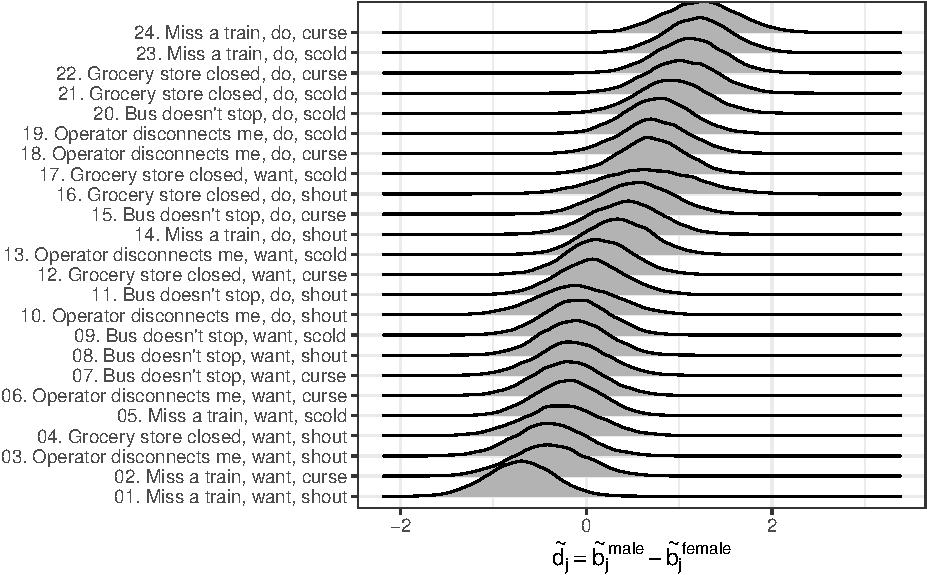
\includegraphics{paper_apa_files/figure-latex/emmilg-1}

}

\caption{GLIMMER for the verbal aggression data. The total performance difference (from either ability differences or DIF), $\tilde{{d_j}}$, for each item is shown. Distributions—as opposed to point estimates—are shown to help the analyst reason about uncertainty. Distributions are calculated by drawing 10,000 imputations from the item parameter covariance matrix. There is no consistent performance difference across items, indicating that the Fundamental DIF Identification Problem is difficult for this data.}\label{fig:emmilg}
\end{figure}

\hypertarget{aimethods}{%
\section{Agnostic Identification Methods}\label{aimethods}}

In this section, we summarize existing AGI methods, propose extensions, and demonstrate their use on the verbal aggression data. So as to offer a coherent framework, we sometimes edit names of existing methods.\footnote{We recognize that others have done the same (e.g., Kopf, Zeileis, \& Strobl, 2015), and that we risk contributing to a proliferation of names.} Recall that the challenge presented by the Fundamental DIF Identification Problem for any AGI method is to disentangle estimation of \(\hat\mu^\text{foc} - \mu^\text{ref} = \hat\mu^\text{foc} - 0 = \hat\mu^\text{foc}\), the difference in mean abilities, from the estimation of \(\hat d_j = \hat{b_j}^{\text{foc}} - \hat{b_j}^{\text{ref}}\), the difference in item easiness. There are two classes of AGI methods. The most common, identification of anchor items, selects a group of items that are assumed to be DIF-free. These anchor items identify the model, thereby allowing for the estimation of \(\hat\mu^\text{foc}\); the remaining items can be tested for DIF using an LRT. The other class involves identification of an anchor point (i.e., directly setting \(\mu^{\text{foc}}\) to some value) (Strobl, Kopf, Hartmann, \& Zeileis, 2018). This anchor point identifies the model, and all items can be tested for DIF using an LRT. We begin by describing anchor item methods.

\hypertarget{anchor-item-methods}{%
\subsection{Anchor Item Methods}\label{anchor-item-methods}}

\hypertarget{all-others-as-anchors-aoaa}{%
\subsubsection{All-others-as-anchors (AOAA)}\label{all-others-as-anchors-aoaa}}

The all-others-as-anchors (AOAA) method tests each item for DIF one at a time using all of the other items as anchors. For example, when testing the first item for DIF, all of the other items are used as anchors. This is done using a LRT that compares the baseline model, where all item parameters are fixed across groups, to the flexible model, where the parameters of the tested item are freed across groups (Thissen, Steinberg, \& Wainer, 1993). Then, when testing the second item for DIF, once again all of the other items (including the first item) are used as anchors, and so on. The items for which the flexible model outperforms the baseline model are identified as having DIF, and the rest of the items become anchor items. AOAA is implemented in the mirt R package, and is called by passing scheme = ``drop'' to the DIF function (drop refers to dropping a single constraint when moving from the baseline to the flexible model).

While some (e.g., Meade \& Wright, 2012) have advocated for the use of AOAA, we note a shortcoming in its key assumption that all items not being tested do not exhibit DIF, which is, of course, counter to the underlying rationale for the undertaking. On a practical level, it is thought that AOAA will perform well if a small minority of items have DIF or the DIF is balanced such that some items are biased against the focal group, while others are biased against the reference group. A simple thought experiment illustrates how AOAA fails: Imagine a three item test where the first item has DIF, and the other two do not. With a sufficiently large number of students, AOAA will find that all items test positive for DIF. The last two items will incorrectly test positive as a result of ``artificial DIF'': Including the first item in the anchor set causes the group ability difference to be misestimated which creates the appearance of DIF in the other two items (Andrich \& Hagquist, 2012).

Figure \ref{fig:aoaa} shows the results of AOAA applied to the verbal aggression data. On the left is the GLIMMER with the curves colored red if AOAA finds the item to contain DIF. In total, AOAA found eight items to contain DIF: Five at the top with more frequent affirmative responses from males and three at the bottom with more frequent affirmative responses from females.\footnote{This is an expected result using AOAA: with a variety of performance differences it tends to find some items with DIF in one direction and other items with DIF in the other direction}. On the right is the final model which is identified by specifying that items without DIF (anchor items) have a difference in item easiness parameters of zero. The final model found \(\hat \mu^\text{male} \approx 0.197\), meaning that males have greater verbal aggression than females on average.\footnote{It can be seen that the final model will estimate \(\mu^\text{male}\) to be positive by noticing that the mean \(\tilde {d_j}\) for anchor items (on the left in the GLIMMER) is positive.}

\begin{figure}[h]

{\centering 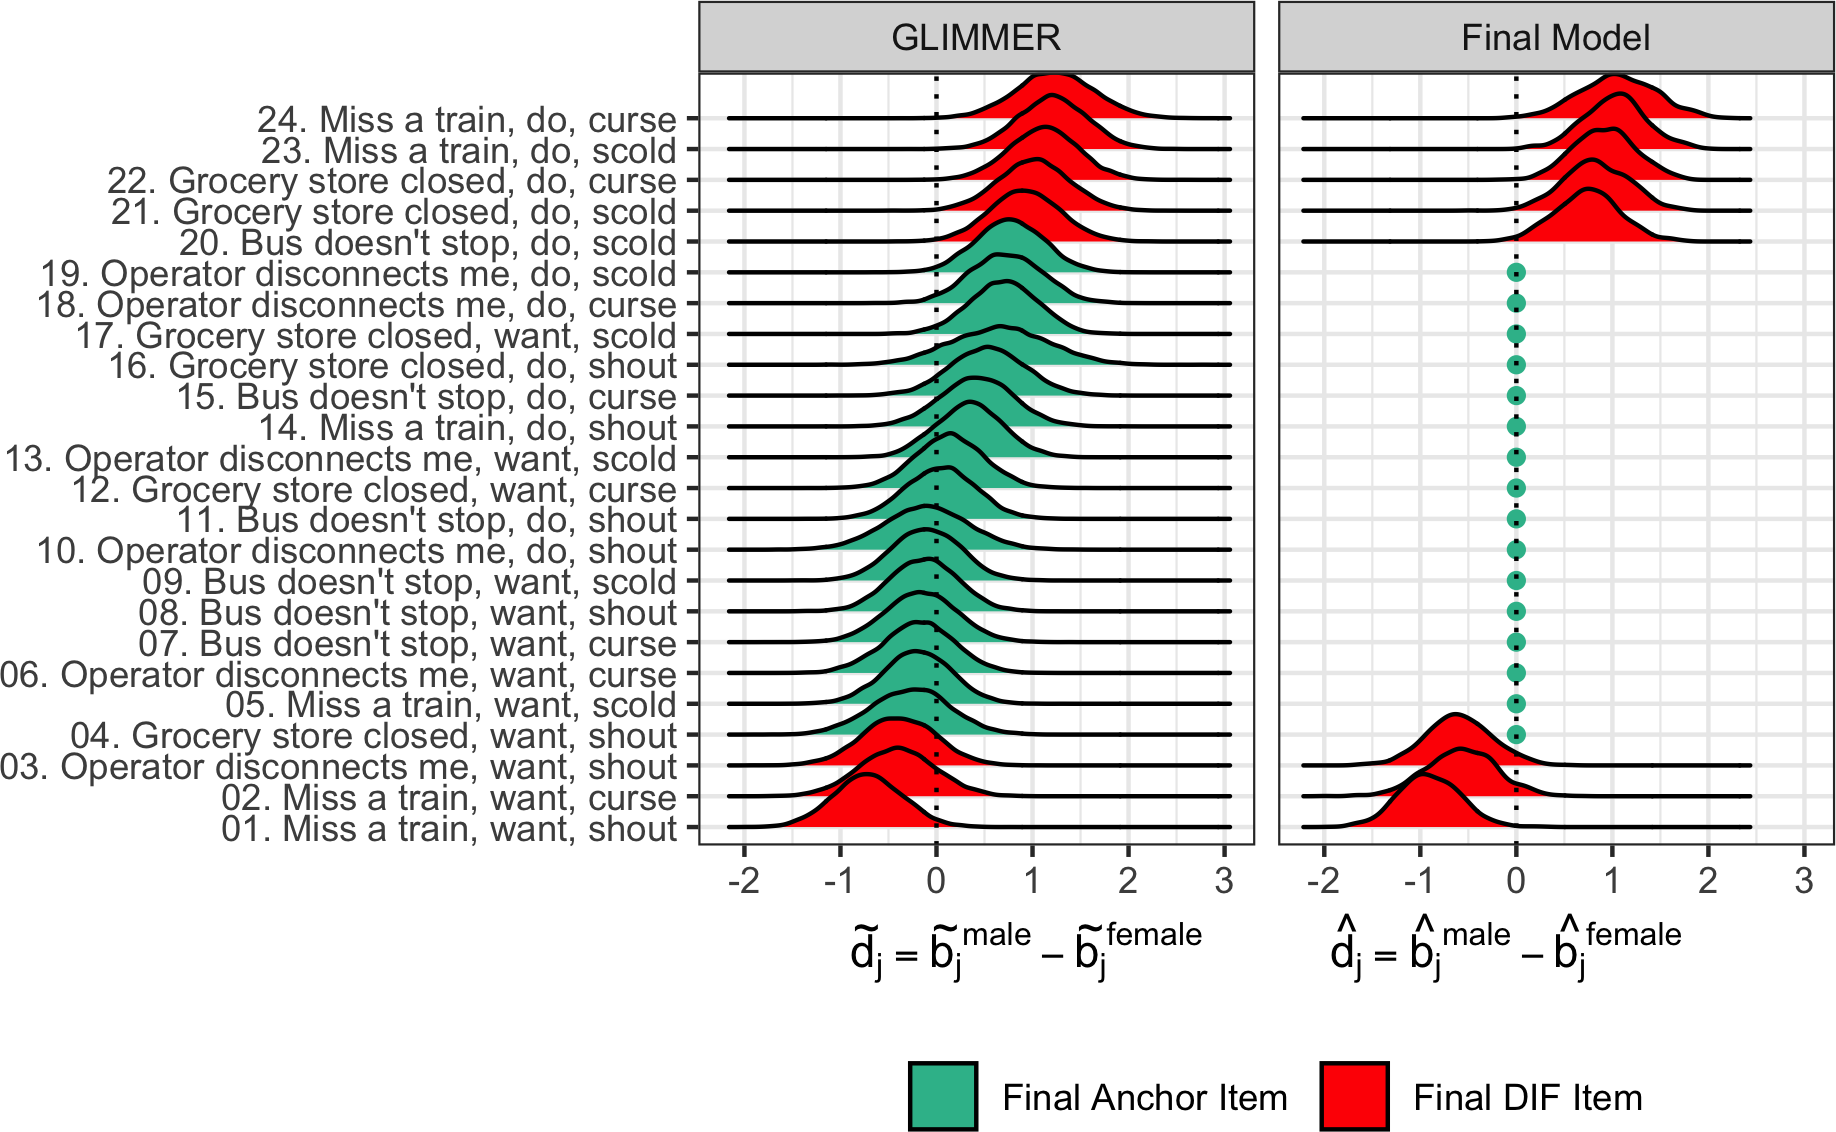
\includegraphics{paper_apa_files/figure-latex/aoaa-1}

}

\caption{AOAA results depicted in a GLIMMER}\label{fig:aoaa}
\end{figure}

\hypertarget{all-others-as-anchors-all-significant-aoaa-as}{%
\subsubsection{All-others-as-anchors-all-significant (AOAA-AS)}\label{all-others-as-anchors-all-significant-aoaa-as}}

One way to attempt to counter artificial DIF is with purification through iterative anchor selection. For example, Drasgow (1987) started with AOAA, removed items displaying DIF from the anchor set, then repeated the process iteratively---with items that have been removed from the anchor set allowed to have free parameters across groups in both the baseline and flexible model---until no more items tested positively. Kopf, Zeileis, and Strobl (2015) named this technique Iterative-backward-AOAA with ``backward'' (as in reverse) referring to beginning with the assumption that all items are DIF-free. We instead refer to this method as all-others-as-anchors-all-significiant (AOAA-AS). We append ``all-significant'' to indicate that all items that test positive for DIF are removed from the anchor set in each iteration. AOAA-AS is implemented in the mirt R package, and is called by passing scheme = ``drop\_sequential'' to the DIF function.

We argue that AOAA-AS, while a potential improvement, doesn't solve the problem of AOAA. The first iteration of AOAA-AS is AOAA. As a result, artificial DIF can still cause items without DIF to test positively for DIF. In the extreme case, what does the analyst do when all items test positively for DIF in the first iteration? Kopf, Zeileis, and Strobl (2015) encountered precisely this problem in their simulation study and chose to select a single anchor item randomly.\footnote{Woods (2009) suggested a more straightforward, one-step method: Use AOAA and select the four items that exhibit the least amount of DIF as anchor items. This method will work in some cases but has the serious limitation of always using exactly four anchor items.} For the verbal aggression data, no additional items tested positive for DIF after the first iteration. Accordingly, the results for AOAA and AOAA-AS are the same as presented in Figure \ref{fig:aoaa}.

\hypertarget{all-others-as-anchors-one-at-a-time-aoaa-oat}{%
\subsubsection{All-others-as-anchors-One-at-a-time (AOAA-OAT)}\label{all-others-as-anchors-one-at-a-time-aoaa-oat}}

We propose an extension of these methods, all-others-as-anchors-one-at-a-time (AOAA-OAT), which, to our knowledge (and surprise), has not previously been explicitly proposed. AOAA-OAT is inspired by Hagquist and Andrich (2017), who assert that ``items showing DIF initially should not be resolved simultaneously but sequentially'' {[}p.~6{]}. Like AOAA-AS, AOAA-OAT starts with AOAA, but only the single item exhibiting the most DIF---based on the \(\chi^2\) test statistic from each LRT---is removed from the anchor set. The process continues iteratively until no new items display DIF. AOAA-OAT and AOAA-AS are similar in that they are both iterative; the difference is that AOAA-OAT takes the more conservative approach of removing only \emph{one} item in each iteration as opposed to \emph{all} items that test positive for DIF. As a result, we believe that AOAA-OAT is less likely to be ``fooled'' by artifical DIF. AOAA-OAT is not currently implemented in the mirt R package.

Figure \ref{fig:aoaaoat} shows the results of AOAA-OAT applied to the verbal aggression data. On the left is the GLIMMER with the curves colored a shade of red or purple according to the order in which they were removed from the anchor set. In total, AOAA-OAT found nine items to contain DIF: The first item removed from the anchor set had more affirmative responses from females than males. The additional eight items removed from the anchor set all had more affirmative responses from males than females. On the right is the final model which is identified by specifying that items without DIF (anchor items) have a difference in item easiness parameter of zero. The final model finds \(\hat \mu^\text{male} \approx 0.001\), meaning that males and females have nearly the same verbal aggression on average.\footnote{It can be seen that the final model will estimate \(\mu^\text{male}\) to be near zero by noticing that the mean \(\tilde {d_j}\) for anchor items (on the left in the GLIMMER) is about zero.} This might seem an odd conclusion: Males score higher on the majority of verbal aggression items, but AOAA-OAT has disregarded many of those items on account of them having DIF. We discuss this issue further when we compare the AGI methods.

\begin{figure}[h]

{\centering 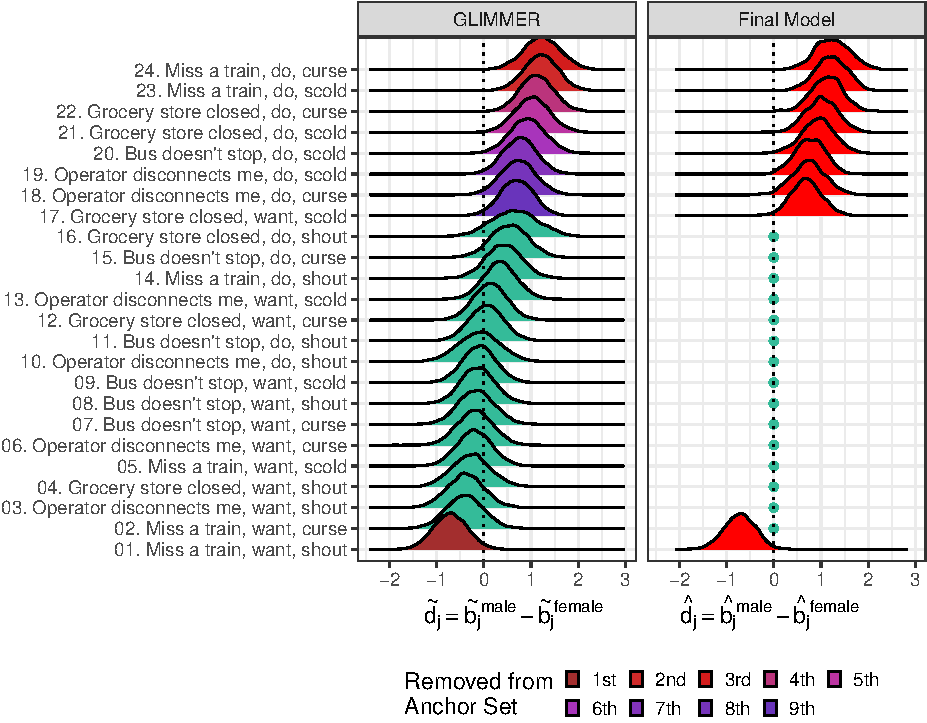
\includegraphics{paper_apa_files/figure-latex/aoaaoat-1}

}

\caption{AOAA-OAT results for the verbal aggression data. On the left, the GLIMMER is identified by setting the group means equal. Green represents items that AOAA-OAT did not find to contain DIF (i.e., anchor items). On the right, the final AOAA model is identified by fixing the anchor items equivalent across groups. Distributions are shown to give a sense of variability and are estimated via 10,000 imputations from the item parameter covariance matrix.}\label{fig:aoaaoat}
\end{figure}

\hypertarget{anchor-point-methods}{%
\subsection{Anchor Point Methods}\label{anchor-point-methods}}

The previously discussed AGI methods identify the model by selecting a set of anchor items that are assumed to be DIF-free. We now discuss the second type of AGI methods: The use of an anchor point (Strobl, Kopf, Hartmann, \& Zeileis, 2018). An anchor point directly sets the difference in mean abilities to some value, \(\mu^{\star\text{foc}}\). Anchor point methods have the advantage of not requiring the assumption that any particular item is DIF-free, and, therefore, allowing all items to be tested for DIF. We describe two methods for selecting the anchor point.

\hypertarget{maximizing-the-gini-index-maxgi}{%
\subsubsection{Maximizing the Gini index (MAXGI)}\label{maximizing-the-gini-index-maxgi}}

Strobl, Kopf, Hartmann, and Zeileis (2018) suggest using the Gini index (Gini, 1912) to select the anchor point. In general, the Gini index ``takes high values if, for example, a small minority of persons has a lot of wealth while the vast majority has very little'' (Strobl, Kopf, Hartmann, \& Zeileis, 2018, p. 7). The Gini index is frequently used to measure the inequality of wealth distribution in a country; for example, South Africa typically has the highest Gini index of all measured countries, meaning that wealth is distributed unevenly (Chitiga, Sekyere, \& Tsoanamatsie, 2015).

Here, DIF effectively takes the role of wealth; Strobl, Kopf, Hartmann, and Zeileis (2018) select \(\mu^{\star\text{foc}}\) by maximizing the Gini index of \(\tilde{\mathbf{d}}\) (thus our abbreviation MAXGI). As a result, models where fewer items are responsible for the majority of deviations from the mean group difference in performance are preferred. Effectively, MAXGI selects the anchor point so that the majority of items having little to no DIF and a small subset of items thus have larger amounts of DIF. Denoting a function that calculates the Gini index from a vector of non-negative elements as \(G(\mathbf{x})\), MAXGI sets
\begin{equation}
\mu^{\star\text{foc}} = \mathop{\mathrm{arg\,max}}_{\mu^\text{foc}} G(|\mu^\text{foc} + \tilde{\mathbf{d}}|)
\end{equation}
where \(\mu^\text{foc} \in (-\infty, \infty)\) and \(\mu^\text{foc}\) is added to each element of \(\tilde{\mathbf{d}}\). For the verbal aggression data, Figure \ref{fig:thegini} shows the gini index at a variety of possible \(\mu^\text{foc}\) values. The result of MAXGI is \(\mu^{\star\text{foc}} = -0.16\).\footnote{There is also a local maximum at \(\mu^{\text{male}} \approx -0.75\), which corresponds to the items that females give affirmative responses to. This illustrates that---as Strobl, Kopf, Hartmann, and Zeileis (2018) point out---the search path is informative.}

\begin{figure}[h]

{\centering 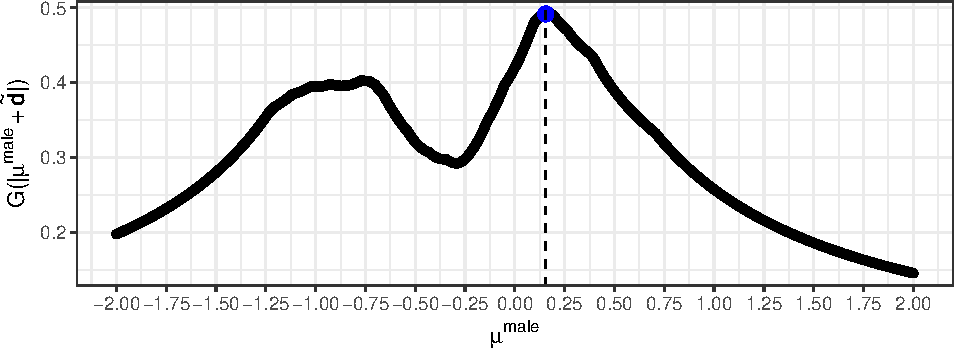
\includegraphics{paper_apa_files/figure-latex/thegini-1}

}

\caption{The search path of MAXGI the verbal aggression data. $\mu^\text{female}$ is fixed to 0 and the goal is to identify the value of $\mu^\text{male}$ that maximizes the gini coefficient. Maximizing the gini coefficient leads to a small minority of items containing DIF.}\label{fig:thegini}
\end{figure}

\hypertarget{minimizing-between-curves-minbc}{%
\subsubsection{Minimizing Between Curves (MINBC)}\label{minimizing-between-curves-minbc}}

We propose an alternative to MAXGI that selects the anchor point by minimizing the total amount of DIF on the test. Accordingly, we name this method ``minimizing between curves'' (MINBC). MINBC is inspired by Raju's area method (Raju, 1988), which measures the amount of DIF by calculating the area between the item characteristic curves, the function that maps the student's ability to their probability of correct response, of the two groups:
\begin{equation}
\text{Area Between Curves} = \int |\text{Pr}(y_j = 1| \theta, b_j^{\text{ref}}) - \text{Pr}(y_j = 1| \theta, b_j^{\text{foc}})| d\theta
\end{equation}
Raju's area method has been cited as one of the most commonly used IRT-based DIF detection methods (Magis, Raiche, Béland, \& Gérard, 2011). However, Raju's area method is not an AGI method because the item characteristic curves first need to be linked. An additional weakness is that the area is typically unweighted, so all values of \(\theta\) within a range---commonly from -6 to 6---matter equally, despite some being much more realistic than others.
MINBC adapts Raju's area method into an AGI method by providing an algorithm for selecting the anchor point. MINBC chooses the anchor point that minimizes the total weighted area between each group's item characteristic curves. It is implemented as follows. We denote \(m(\mu^\text{foc})\) to be a function that takes \(\mu^\text{foc}\) as input and estimates \(\hat b_j^\text{foc}\) by fitting a unidimensional Rasch model. The amount of DIF on each item is calculated as
\begin{equation}
\text{DIF}_j(\mu^\text{foc}) = \int |\text{Pr}(y_j = 1| \theta, b_j^{\text{ref}}) - \text{Pr}(y_j = 1| \theta, m_j(\mu^\text{foc}))| g(\theta)d\theta
\end{equation}
where \(g(\theta)\) is a weighting function such that \(\int g(\theta)d\theta = 1\). \(\text{Total DIF}(\mu^\text{foc})\) is a function where the input is \(\mu^\text{foc}\) and the output is the total amount of DIF on the test:
\begin{equation}
\text{Total DIF}(\mu^\text{foc}) = \sum_{j} \text{DIF}_j(\mu^\text{foc}).
\end{equation}
MINBC sets the anchor point to be the value of \(\mu^{\star\text{foc}}\) that minimizes the total amount of DIF on the test:
\begin{equation}
\mu^{\star\text{foc}} = \mathop{\mathrm{arg\,min}}_{\mu^\text{foc}} \text{Total DIF}(\mu^\text{foc}).
\end{equation}
MINBC is inspired in part by Chalmers, Counsell, and Flora (2016), who use the difference between test characteristic curves weighted by \(g(\theta)\) as a measure of differential test functioning (DTF). The selection of \(g(\theta)\) results in the relative weighting of \(\theta\) values. Chalmers, Counsell, and Flora do not discuss how to choose \(g(\theta)\) and in their empirical examples use \(g(\theta)\) uniform for \(-6 \le \theta \le 6\), which may be suboptimal in some cases. It might seem intuitive to choose \(g(\theta) \sim N(0, 1)\) because \(\mu^\text{female} = 0\), but this choice doesn't take into account the ability distribution of the focal group. For example, if \(\mu^\text{foc} = 3\), we would want to prioritize higher \(\theta\) values. Based on this logic, we set \(g(\theta)\) to be the weighted average of the reference and focal group ability probability density functions:
\begin{equation}
g(\theta) = p^\text{ref} \cdot N(\mu^{\text{ref}}, \sigma^{\text{ref}^2}) + (1 - p^\text{ref}) \cdot N(\mu^{\text{foc}}, \sigma^{\text{foc}^2}).
\end{equation}

To understand MINBC, imagine a scenario in which the data-generating process is \(\mu^{\text{foc}} = \mu^{\text{ref}}\) and \(d_j = 0 \forall j\), so that the groups have equal ability and there is no DIF. The Fundamental DIF Identification Problem is that there are an infinite number of models with the same likelihood from which to choose. For example, we could correctly assume that the focal group has the same ability as the reference group and fix \(\mu^{\star\text{foc}} = 0\). The model would then estimate \(\hat d_j \approx 0 \forall j\), and we would correctly conclude the groups have the same ability and there is no DIF. Alternatively, we could assume that the focal group has \(\mu^{\star\text{foc}} = 3\). The model would then compensate by finding \(\hat d_j \approx -3 \forall j\), and we would incorrectly conclude that the focal group is high ability, but every item contains DIF against them. Both of these models have the same likelihood, so how should one choose which model to believe? MINBC chooses the model with the least amount of total DIF, as measured by the total weighted area between the item characteristic curves. As a result, the likelihood tie is broken by preferring to explain differences in performance across groups by ability differences (as opposed to DIF). Figure \ref{fig:minbc} shows Total DIF at a variety of possible values for \(\mu^\text{male}\). The result is \(\hat \mu^\text{male} \approx 0.34\).

\begin{figure}[h]

{\centering 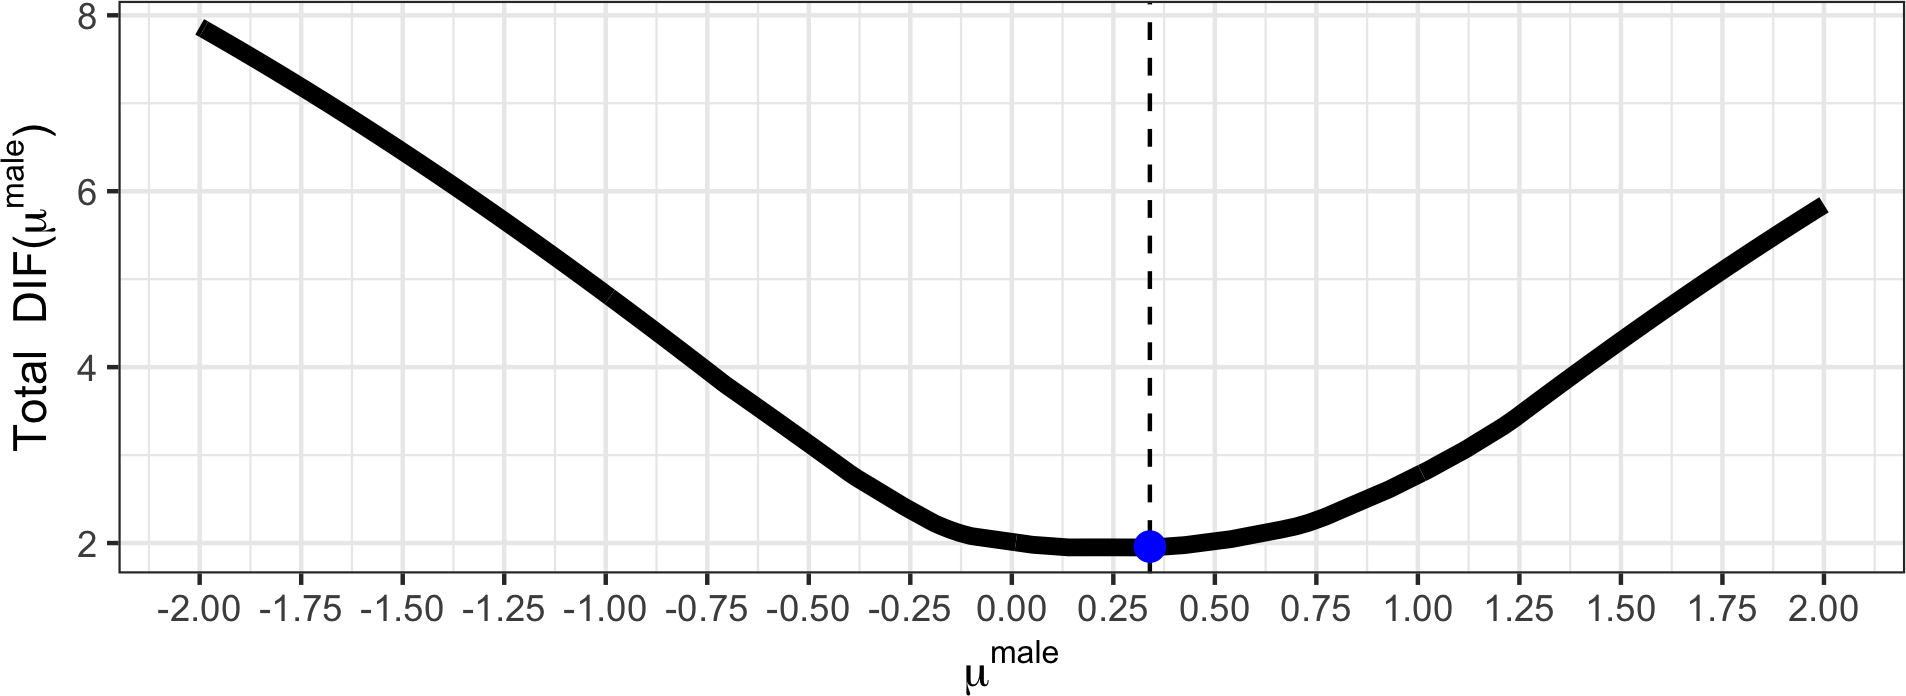
\includegraphics{paper_apa_files/figure-latex/minbc-1}

}

\caption{The search path of MINBC for the verbal aggression data. $\mu^\text{female}$ is fixed to 0 and the goal is to identify the value of $\mu^\text{male}$ that minimizes the total area between item characteristic curves. As a result, the total amount of DIF on the test is minimized and as much performance difference as possible is explained by group ability differences.}\label{fig:minbc}
\end{figure}

\hypertarget{comparing-methods}{%
\subsection{Comparing Methods}\label{comparing-methods}}

We described a variety of AGI methods. Anchor item methods---AOAA, AOAA-AS, and AOAA-OAT---address the Fundamental DIF Identification Problem by assuming a set of items do not contain DIF. Anchor point methods---MAXGI and MINBC---implement a rule to directly find group latent trait means.

Each of these methods implemented an (arguably) reasonable algorithm to identify the final item response model. These final item response models each contain an estimate of the male-female group difference in verbal aggression, which are shown as vertical lines in Figure \ref{fig:summary}. Figure \ref{fig:summary} reveals that the conclusions arrived at vary significantly by DIF detection method. If the analyst were to use AOAA-OAT, they would find that males and females have nearly the same verbal aggression on average. On the other hand, if they were to use MINBC, they would find that males have significantly greater verbal aggression than females. A natural question to ask is, which AIG method is right? Instead of one method being best---which DIF detection method research has searched long and hard for---the variety of results is a consequence of the Fundamental DIF Identification Problem being fraught for the verbal aggression data as shown by the geometry of the GLIMMER in Figure \ref{fig:emmilg}. This is evidence that none of the AGI methods should be fully trusted.

\begin{figure}[h]

{\centering 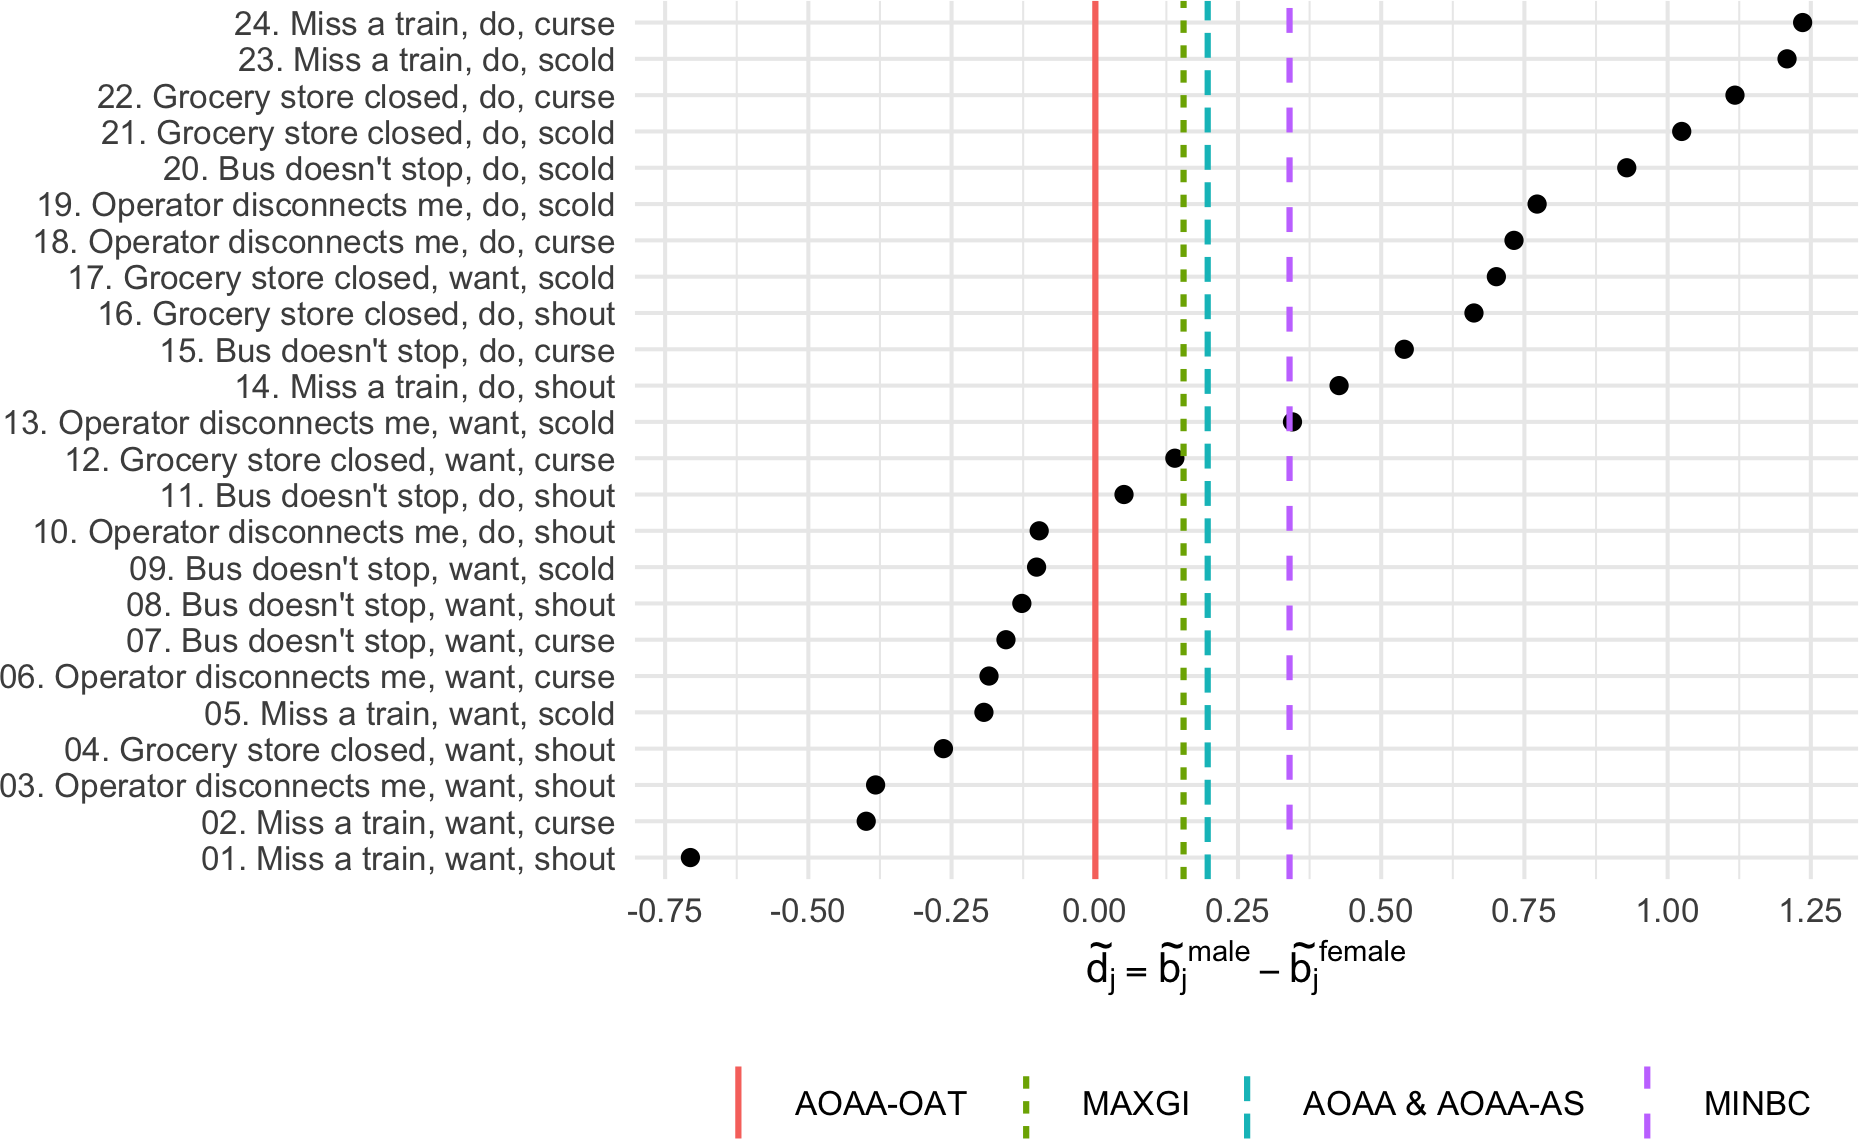
\includegraphics{paper_apa_files/figure-latex/summary-1}

}

\caption{Results by DIF detection method. The male group mean verbal aggression, $\hat \mu^\text{male}$, according to each method is graphed as a vertical line, which are superimposed over the performance difference, $\tilde {d_j}$, for each item. The scale is set by fixing $\hat \mu^\text{female} = 0$.}\label{fig:summary}
\end{figure}

\hypertarget{simulation-study}{%
\section{Simulation Study}\label{simulation-study}}

The verbal aggression data provided an example of how AGI methods can lead to different conclusions. However, being real-world data, we cannot know the data generating processes underlying the differences that we observed. And, as a consequence, we could not adjudicate between methods. To illustrate the AGI methods' performance when the data generating model is known, we conducted a simulation study. Within the simulation study, we were able to measure the performance of each AGI method, but it's critical to note out at the outset that a simulation study can only conclude that a method is best under specific conditions, not in general.

The majority of DIF simulation studies in the literature generate data by simply altering the item easiness parameters for the focal group (e.g., setting the focal group's item easiness parameter to the reference group's item easiness parameter minus a constant). As described in the appendix, this setup views DIF as a property of the item that equally impacts all students from the same group. We find it more realistic to think of DIF as the result of each item tapping into a secondary ability to a varying degree. For example, Ackerman (1992) describe a scenario in which some items on a math test depend on both a student's math ability (the target ability) and the student's verbal ability (the nuisance ability).

\hypertarget{data-generating-model}{%
\subsection{Data Generating Model}\label{data-generating-model}}

Our simulation study was inspired by Walker and Gocer Sahin (2017) who conducted a series of simulations to determine how high the correlation between the target and nuisance abilities must be for DIF to undetectable. Unlike Walker and Gocer Sahin (2017), we used a noncompensatory item response model where an individual cannot compensate for being low on the nuisance ability by being relatively high on the target ability. Ackerman (1992)'s scenario of a math test may be an example of a case where a noncompensatory model is realistic: Perhaps a student's math ability is largely irrelevant when they encounter a word problem that they cannot parse. In particular, we generated item responses using an adapted version of Sympson's (1978) noncompensatory item response model in which
\begin{equation}
\text{Pr}(y_{ij} = 1 | \theta_i, \eta_i, a_{\eta j}) = \sigma(\theta_i + b_{\theta j}) \cdot \sigma(a_{\eta j}\eta_i + b_{\eta j})
\end{equation}
where \(\theta_i\) and \(\eta_i\) is individual \(i\)'s target ability and nuisance ability, respectively; \(a_{\eta j}\) is item \(j\)'s loading on nuisance ability; and \(b_{\theta j}\) and \(b_{\eta j}\) are item \(j\)'s target easiness and nuisance easiness, respectively (DeMars, 2016).

Each test had 12 items, and we used five conditions corresponding to two, three, four, five, and six DIF items. For items without DIF (i.e., that don't depend on the nuisance ability), we set \(b_{\eta j} = \infty\) and \(b_{\theta j} = 0\) which resulted in the model reducing to \(\text{Pr}(y_{ij} = 1) = \sigma(\theta_i)\). For items with DIF (i.e., that depend on the nuisance ability), we chose relatively high item easiness parameters---\(b_{\theta j} = 2\) and \(b_{\theta j} = 2\)---so that the overall probability after multiplying the two sigmoid functions together was similar for items with and without DIF. This choice resulted in the model reducing to \(\text{Pr}(y_{ij} = 1) = \sigma(\theta_i + 2) \cdot \sigma(a_{\eta j}\eta_i + 2)\). For items with DIF, \(a_{\eta j}\) was calculated by adapting Ackerman's (1994) angle equation as described in Walker and Gocer Sahin (2017):
\begin{equation}
\angle_j = \arccos \dfrac{1}{1 + a_{\eta j}^2}.
\end{equation}
An item's angle measures the relative loading of the item on the two dimensions. The lower the angle, the more the item loads on target ability as compared to nuisance ability, which corresponds to less DIF. An angle of 45\(^\circ\) indicates that the item loads equally on the target ability and nuisance ability. We were interested in specifying the angle of an item, so the relevant equation became
\begin{equation}
a_{2j} = \sqrt{\dfrac{1 - \cos(\angle_j)^2}{\cos(\angle_j)^2}}.
\end{equation}
For DIF items, we set \(a_{\eta j}\) based on angles with equal intervals between 20\(^\circ\) and 60\(^\circ\). For example, for a test with three DIF items, the angles are 20\(^\circ\), 40\(^\circ\), and 60\(^\circ\).

We conducted 100 replications for each of the five conditions. In each replication, we simulated 10,000 students with half coming from each of the reference and focal groups. For students from the reference group, target ability and nuisance ability were drawn from the two-dimensional normal distribution with mean {[}\(\mu_\theta^\text{ref} = 0\), \(\mu_\eta^\text{ref} = 0\){]} and covariance matrix \(\begin{bmatrix} 1 & 0.5 \\ 0.5 & 1 \end{bmatrix}\). Abilities for students from the focal group were drawn using the same covariance matrix, but with means {[}\(\mu_\theta^\text{foc} = -0.5\), \(\mu_\eta^\text{foc} = -1\){]}. In summary, the focal group had a lower mean target ability and a lower mean nuisance ability; it's the goal of a DIF detection process to result in unbiased measurement of the target ability.

Figure \ref{fig:difmap} provides intuition about the data generating model by showing the relationship between \(\theta_i\) and \(\text{Pr}(y_{ij} = 1)\) (i.e., item characteristic curves) with \(\eta_i\) set to the group mean for a test with six items with DIF. The items are ordered by the amount of DIF such that \(\angle_{j = 7} = 20^\circ\) up to \(\angle_{j = 12} = 60^\circ\). In essence, the two groups had the same relationship with items one through six as those items did not load on \(\eta_i\). The last six items contained increasing amounts of DIF against the focal group as those items loaded on \(\eta_i\).

\begin{figure}[h]

{\centering 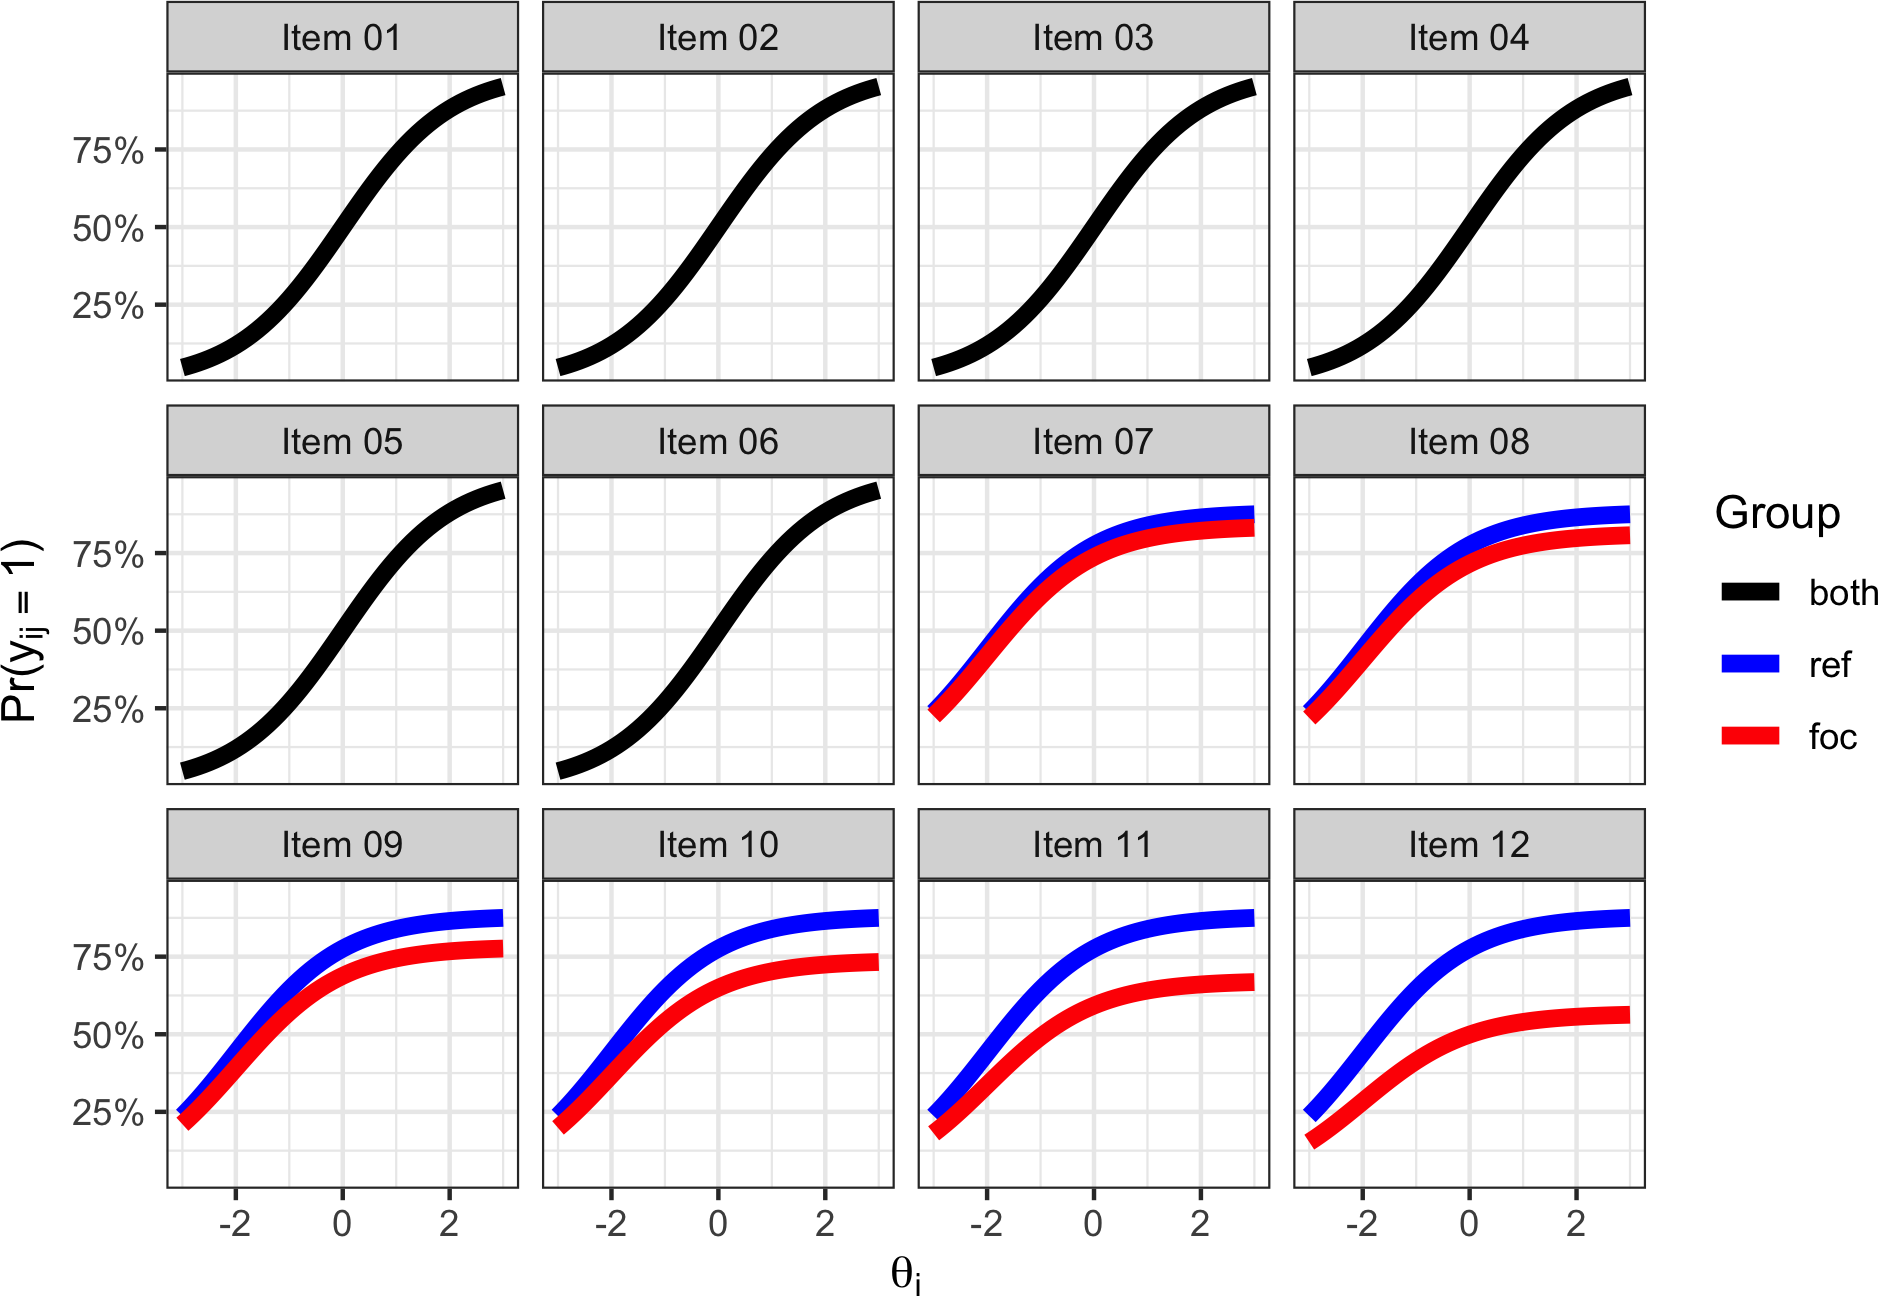
\includegraphics[width=1\linewidth]{paper_apa_files/figure-latex/difmap-1}

}

\caption{The relationship between target ability and probability of correct response for a 12-item test where the last 6 items contain DIF. Nuisance ability is fixed to the group mean. The reference group has the same item characteristic curve for each item; the focal group has lower probabilities of correct responses the more the item requires the nuisance ability.}\label{fig:difmap}
\end{figure}

We now describe the analysis methods that we took. We sequence these in two steps---first, inspect a GLIMMER and second, execute and compare the results from multiple AGI methods---so as to mirror our recommended DIF detection process for an analyst confronted with a single data set. Each of the analysis methods involve fitting the multigroup Rasch model (see equation \ref{eq:rasch}). Computing was done in R (R Core Team, 2019), model fitting in the mirt R package (Chalmers, 2012), and data wrangling/visualization in the suite of R packages known as the tidyverse (Wickham, 2017). Code is available at \emph{BLINDED}.

\hypertarget{step-1-create-a-glimmer}{%
\subsection{Step 1: Create a GLIMMER}\label{step-1-create-a-glimmer}}

Figure \ref{fig:difmap} requires knowledge of the data generating model, and is therefore unavailable to the analyst. The next best thing is a GLIMMER, which allows the analyst to visualize the performance differences on each item. We suggest that the analyst begins DIF detection by looking at a GLIMMER. As an example, Figure \ref{fig:simemmlg} shows the GLIMMER for one replication using the same item parameters that generated Figure \ref{fig:difmap}. As a reminder, a GLIMMER is generated by fixing both group means to 0 so that all performance differences manifest in the free estimation of the item easiness parameters. As expected, \(\tilde{d_j}\) is consistent for the first six items which do not contain DIF. Further, for the last six items, \(\tilde{d_j}\) increases as \(\angle_j\) increases. From inspecting the GLIMMER, the analyst might (correctly) assume that the first six items can be used as anchors. In general, the analyst should be reassured to by a GLIMMER that shows consistent differences across items.

\begin{figure}[h]

{\centering 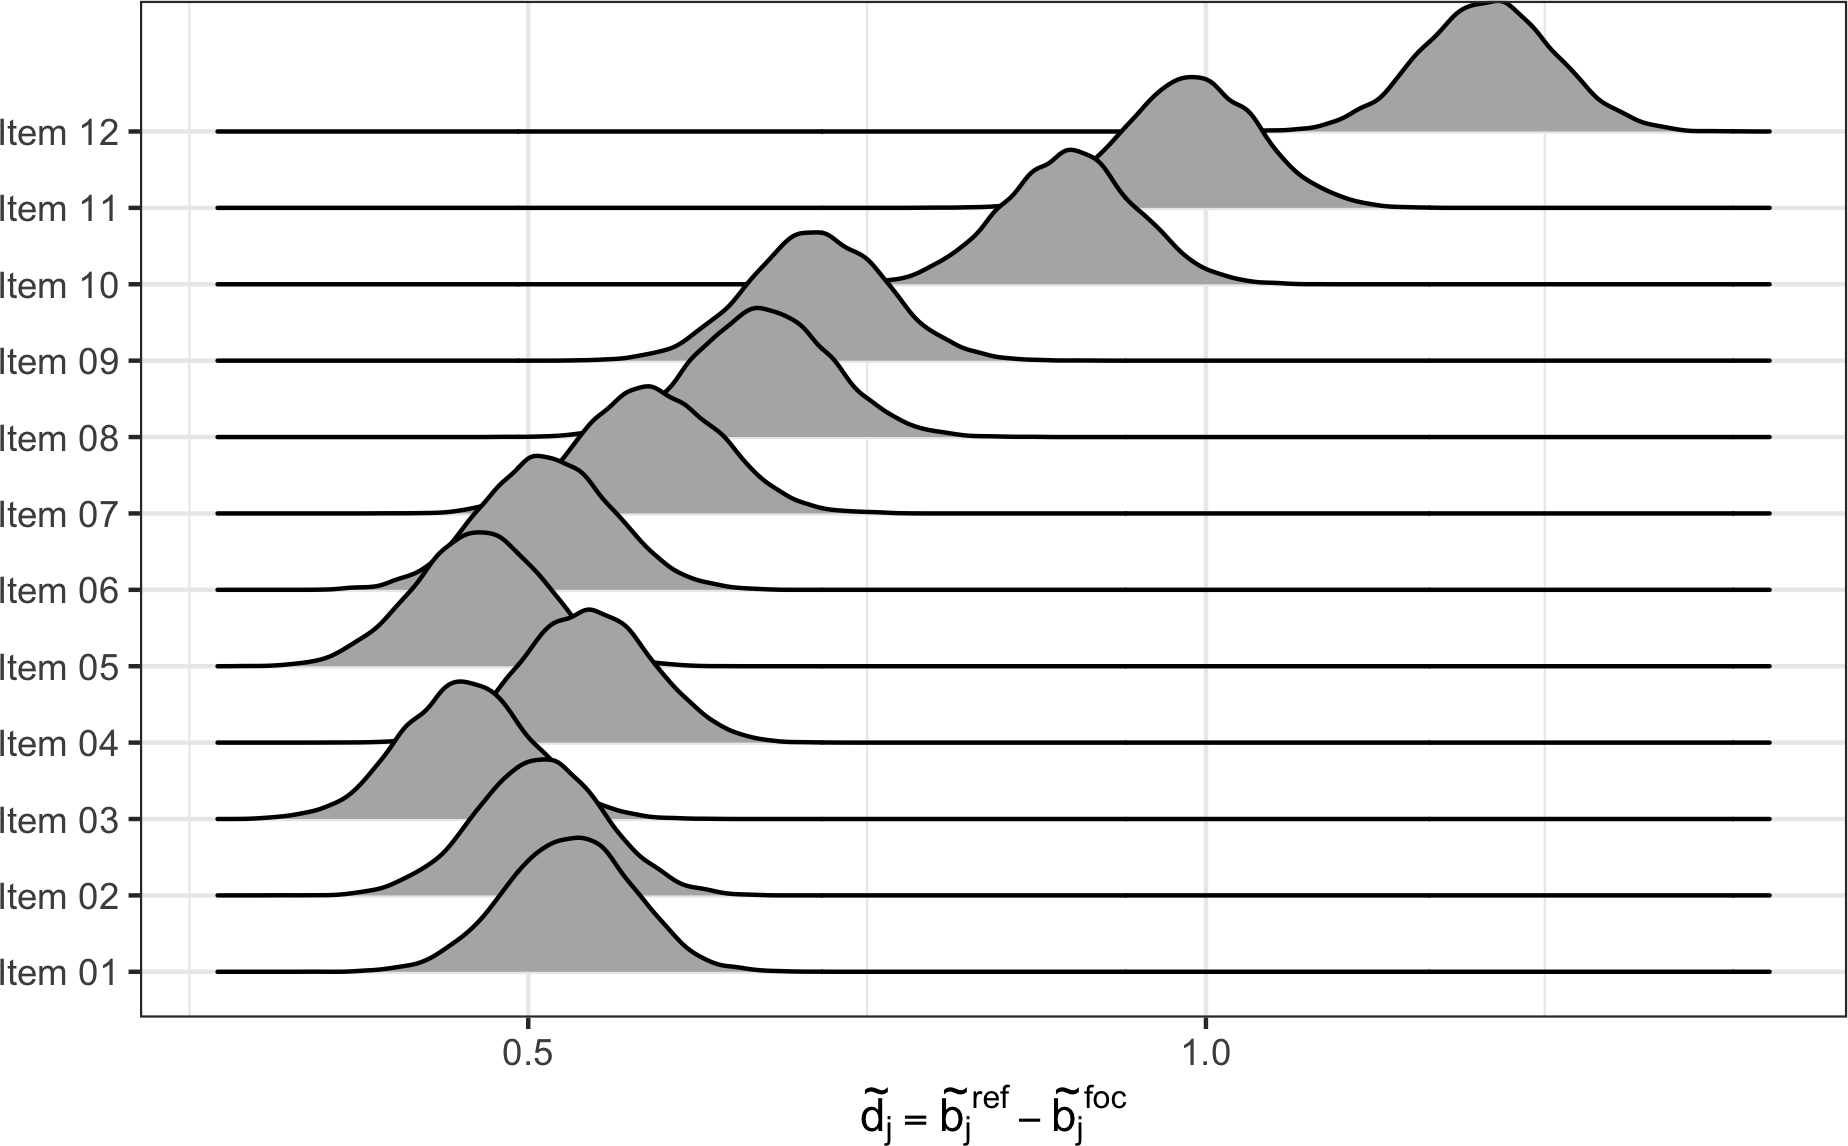
\includegraphics[width=0.7\linewidth]{paper_apa_files/figure-latex/simemmlg-1}

}

\caption{GLIMMER for one replication using the same item parameters as generated Figure \ref{fig:difmap}. The six DIF-free items (items 1-6) show a constant performance difference. As expected, the other six items (items 7-12) show an increasingly large performance difference.}\label{fig:simemmlg}
\end{figure}

\hypertarget{step-2-compare-multiple-agi-methods}{%
\subsection{Step 2: Compare Multiple AGI Methods}\label{step-2-compare-multiple-agi-methods}}

After inspecting a GLIMMER, our second suggested step for DIF detection is to compare performance across multiple AGI methods. Of course, the analyst will typically be working with a single data set and will not know the true data generating model. Here, we implemented a simulation study version of this step by comparing the performance of each of the AGI methods across each of the replications. In particular, we applied each AGI method to find the method's identifying assumption. The method's identifying assumption was then used to fit a final model. We compared the performance of those final models according to the following outcomes.

\textbf{Anchor Item Detection:} For the methods that choose a set of anchor items, we looked directly at which anchor items were selected. An effective method should use most of the non-DIF items as anchors (the anchor hit rate) while avoiding using items with DIF as anchors (the DIF avoidance rate).

\textbf{Achievement Gap Residual:} An effective AGI method should lead to a final model that accurately estimates the difference between the reference group's mean target ability and the focal group's mean target ability. We refer to this quantity as the achievement gap. Recall that all models set \(\mu_\theta^\text{ref} = 0\), so the achievement gap reduces to \(\mu_\theta^\text{foc}\). The data-generating value of \(\mu_\theta^\text{foc}\) is 0.5, but each replication, of course, includes sampling variability. To get at the heart of how well a method is doing, we calculated the achievement gap residual as the method's estimated achievement gap, \(\hat\mu_\theta^\text{foc}\), minus the achievement gap estimated when using only the DIF-free items as anchors. In summary, this outcome measures a method's ability to disentangle differences in target ability from nuisance ability at the group level.

\hypertarget{results}{%
\subsubsection{Results}\label{results}}

AOAA-OAT performed much better at correctly identifying anchor items than AOAA-AS and AOAA. The anchor item detection results are shown in Figure \ref{fig:anchorfalse}. As shown in the top row, AOAA-OAT remarkably included an average of over \(90\%\) of DIF-free items in the anchor set regardless of the number of DIF items on the test. Conversely, AOAA-AS and AOAA had significant performance degradation for conditions with more DIF items. As shown in the bottom row, each method performed similarly in terms of DIF avoidance rate. By inspecting several of the replications we observed a pattern that makes sense given the GLIMMER's geometry (see Figure \ref{fig:simemmlg}): AOAA-OAT tended to remove the items with DIF one by one, starting with the item with the most severe DIF (the largest angle). The only mistake that AOAA-OAT frequently made was failing to flag the item with 20\(^\circ\) of DIF in its last iteration. AOAA-AS and AOAA fared much worse: Both methods tended to result in an anchor set comprised exclusively of the items with 20\(^\circ\) and 40\(^\circ\) of DIF. In most replications, AOAA-AS stopped after one or two iterations, which explains why AOAA and AOAA-AS had similar results.

\begin{figure}[h]

{\centering 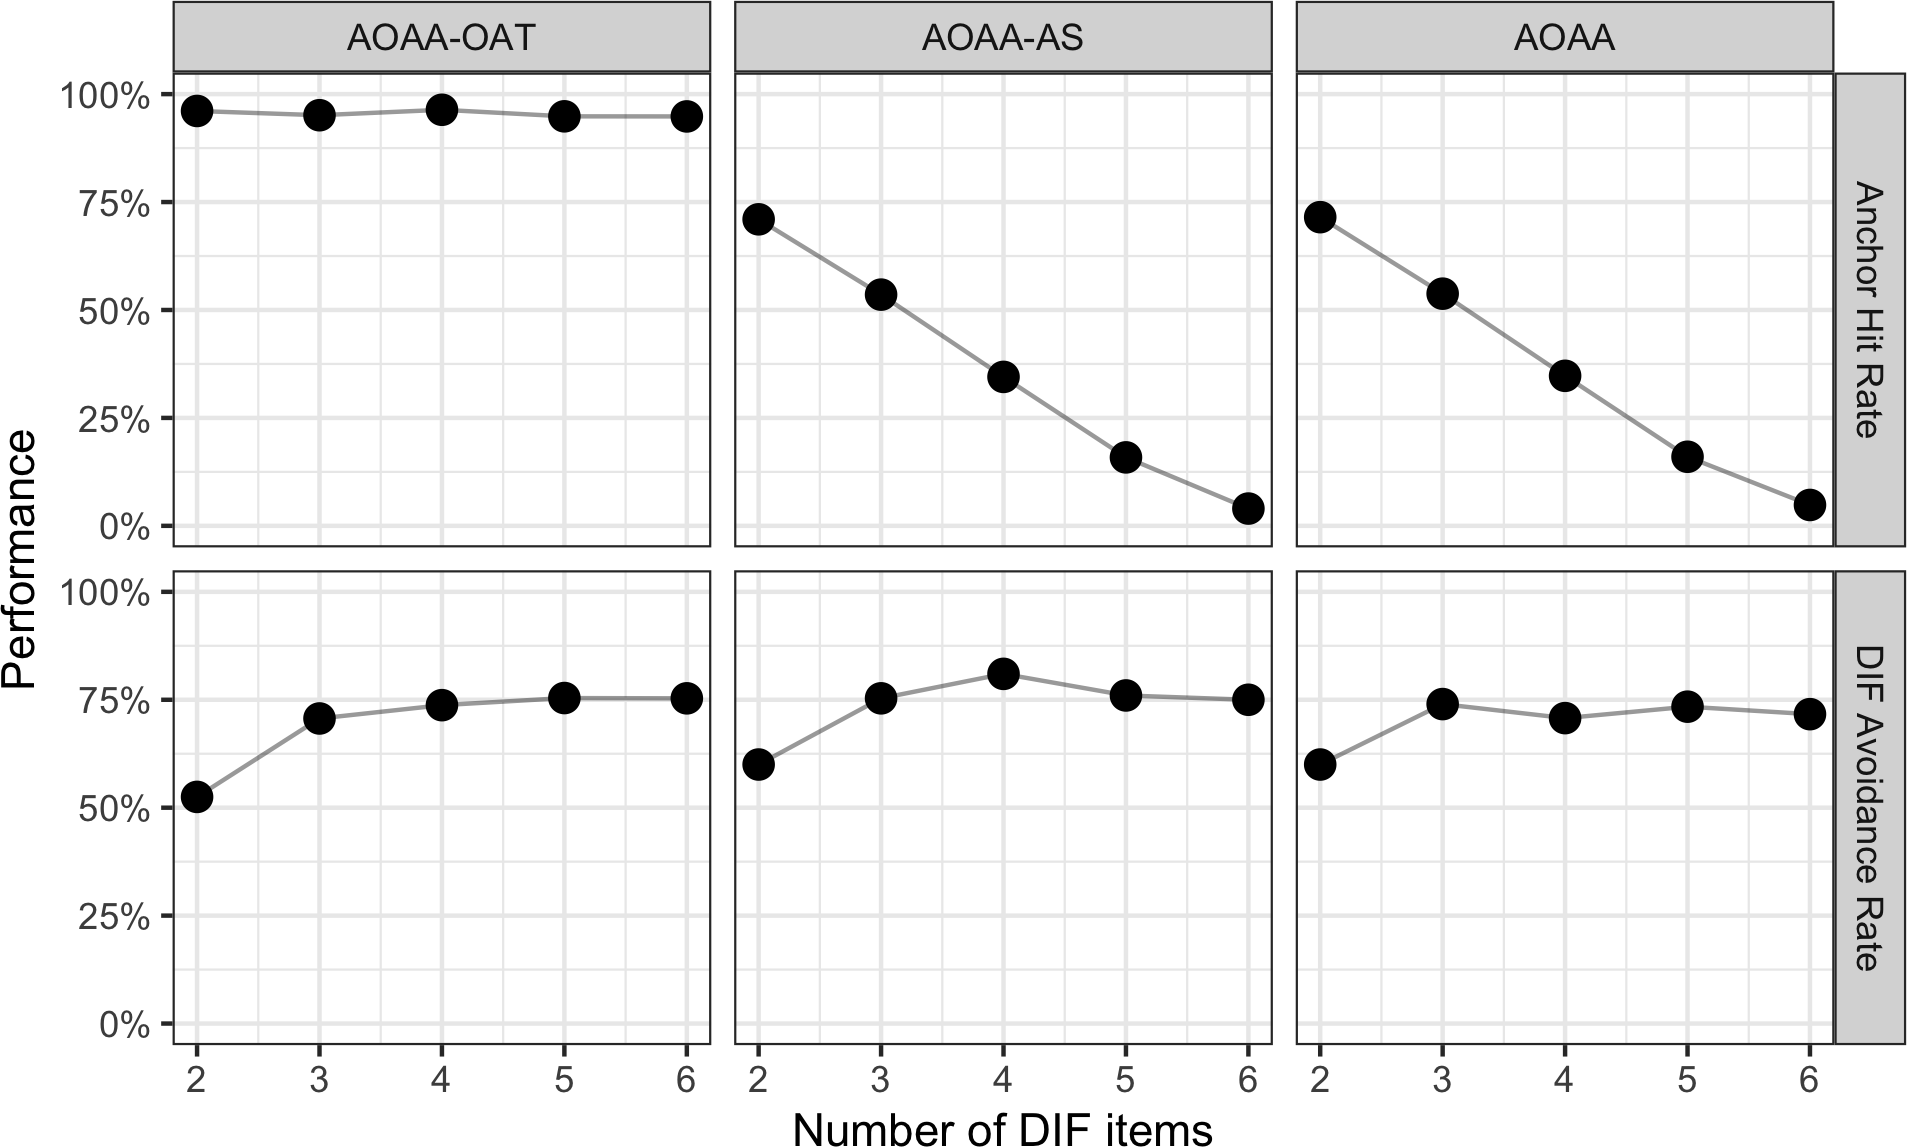
\includegraphics{paper_apa_files/figure-latex/anchorfalse-1}

}

\caption{Performance rates across 100 replications for each AGI method and number of DIF items. Top row: AOAA-OAT nearly always chooses all of the non-DIF items as anchors (the anchor hit rate) while AOAA-AS and AOAA do much better for fewer DIF items. Bottom row: All of the methods perform similarly as far as avoiding including items with DIF in the anchor set (DIF avoidance rate). DIF avoidance rates are slightly lower for the two DIF item condition because the item with 20$^\circ$ of DIF was frequently incorrectly included in the anchor set (and it was one of only two items with DIF in this condition).}\label{fig:anchorfalse}
\end{figure}

Ultimately, the goal of an item response model is often not to flag items containing DIF but rather to measure some property of the respondents without bias. One such possibility is the difference in group means which we have encapsulated in the achievement gap residual. Figure \ref{fig:achievegap} shows each method's performance on the achievement gap residual. AOAA-OAT was the clear winner. It performed nearly flawlessly for two, three, or four DIF items. Even when six of the 12 items on the test contained DIF, AOAA-OAT underestimated \(\mu_\theta^\text{foc}\) by only 0.07 standard deviations on its worst replication. As expected, artificial DIF caused AOAA and AOAA-AS to exhibit problematic performance in conditions with more than three DIF items increased. MINBC and MAXGI performed similarly well with MINBC estimating the achievement gap with more precision but more bias than MAXGI, especially for tests with more than four DIF items. We hypothesize that MINBC's susceptibility to bias results from considering every item. AOAA-OAT, on the other hand, completely disregards an item once it's removed from the anchor set.

\begin{figure}[h]

{\centering 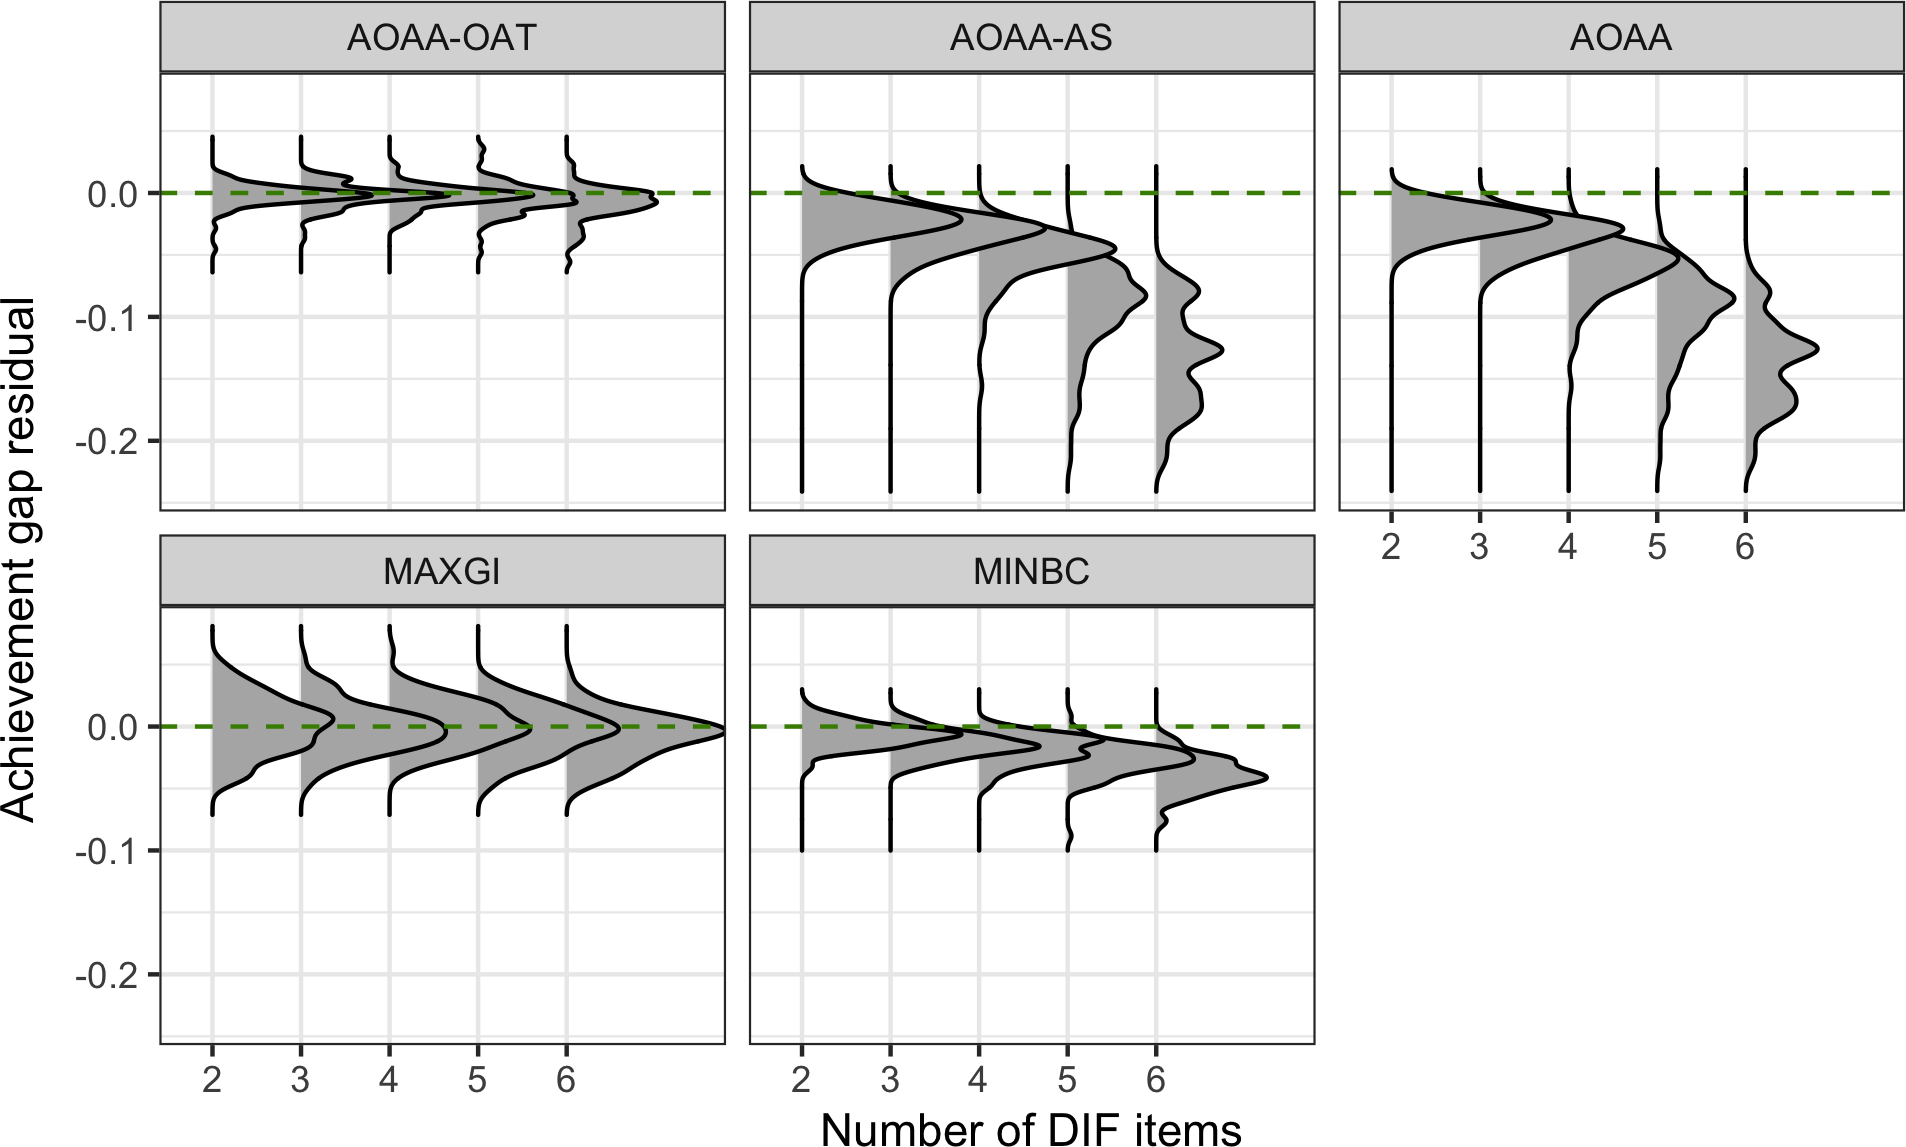
\includegraphics{paper_apa_files/figure-latex/achievegap-1}

}

\caption{Achievement gap residual distributions across 100 replications for each AGI method and number of DIF items.}\label{fig:achievegap}
\end{figure}

\hypertarget{discussion}{%
\section{Discussion}\label{discussion}}

Validity hinges on measurement instruments being relatively free of DIF (Bryant, 2000). Such instruments need to be inspected for DIF so that we can be sure of the validity of the conclusions that we draw regardless of the group membership of each respondent. At the beginning of most DIF detection is a particularly difficult problem that we have referred to as the Fundamental DIF Identification Problem. This problem is typically tackled implicitly by DIF methods---during what we have called agnostic identification (AGI)---with the analyst sometimes lacking awareness of its existence. As a result, some applied DIF studies report certainly conclusions that rest on tenuous assumptions.

In other words, one of our main concerns is that the analyst can be lulled into a false sense of security: The analyst chooses a method, implements it, and then proceeds as if the method certainly resulted in a model that reflects some objective reality. The classic verbal aggression data provides a powerful example: Our results showed that different methods lead to significantly different conclusions. We argue that this is because the Fundamental DIF Identification Problem is unsolvable for the verbal aggression data. Further, we conducted a simulation study where some items (i.e., the DIF-free items) loaded exclusively on target ability while other items (i.e., the DIF items) loaded on both target and nuisance ability. Mirroring our suggested DIF detection process, we showed an example of how a GLIMMER can give the analyst insight into the data generating process. We then compared each of the AGI methods in terms of their ability to correctly identify anchor items. AOAA-OAT exhibited superior performance, which is an important finding given that it is, to our knowledge, not used currently. We advocate for its widespread use as part of any DIF detection process. One drawback of the AOAA-OAT method is that it is computationally expensive. For example, finding three items containing DIF on a 12-item test requires fitting 46 item response models, and that number grows as either the test length or the number of items testing positive for DIF grows. However, we believe the computational costs are worthwhile. To increase AOAA-OAT's use, we recommend its implementation (perhaps as the default) in popular IRT software such as the mirt R package.

In general, we suggest the following process for DIF detection. First, examine raw item response data for potential DIF. To this end, the GLIMMER combats this concern by presenting all information clearly to the analyst. The GLIMMER has the following advantages to this end: (a) By arbitrarily setting the group means equal, the GLIMMER remains agnostic to an identification assumption; (b) by using multiple imputations, the GLIMMER allows for understanding sampling variability/statistical significance; and (c) by using MMLE, the GLIMMER appropriately handles missing responses. Second, use and compare the results from multiple AGI methods. We demonstrated this process using the classic verbal aggression data, which highlighted just how sensitive DIF results can be to method. This is an important point given that most applied DIF studies use a single method and seem to give little consideration to the choice of that method. Third, understand the possible failure of DIF methods and report results as being contingent on assumptions.

In closing, future work should test these methods' performance under a greater variety of data generating conditions. For example, changing the compensatory nature of the data generating model or adding additional nuisance ability dimensions. Finally, our work focused on the Rasch model, and it is of great interest to consider how these methods extend and perform when the goal is to detect and correct for DIF in the context of more flexible item response models.

\clearpage

\hypertarget{references}{%
\section{References}\label{references}}

\begingroup
\setlength{\parindent}{-0.5in}
\setlength{\leftskip}{0.5in}

\hypertarget{refs}{}
\begin{CSLReferences}{1}{0}
\leavevmode\hypertarget{ref-ackerman1992didactic}{}%
Ackerman, T. A. (1992). A didactic explanation of item bias, item impact, and item validity from a multidimensional perspective. \emph{Journal of Educational Measurement}, \emph{29}(1), 67--91.

\leavevmode\hypertarget{ref-ackerman1994using}{}%
Ackerman, T. A. (1994). Using multidimensional item response theory to understand what items and tests are measuring. \emph{Applied Measurement in Education}, \emph{7}(4), 255--278.

\leavevmode\hypertarget{ref-amtmann2010development}{}%
Amtmann, D., Cook, K. F., Jensen, M. P., Chen, W.-H., Choi, S., Revicki, D., \ldots{} others. (2010). Development of a PROMIS item bank to measure pain interference. \emph{Pain}, \emph{150}(1), 173--182.

\leavevmode\hypertarget{ref-andrich2012real}{}%
Andrich, D., \& Hagquist, C. (2012). Real and artificial differential item functioning. \emph{Journal of Educational and Behavioral Statistics}, \emph{37}(3), 387--416.

\leavevmode\hypertarget{ref-angoff1993perspectives}{}%
Angoff, W. H. (1993). Perspectives on differential item functioning methodology.

\leavevmode\hypertarget{ref-bock1981marginal}{}%
Bock, R. D., \& Aitkin, M. (1981). Marginal maximum likelihood estimation of item parameters: Application of an EM algorithm. \emph{Psychometrika}, \emph{46}(4), 443--459.

\leavevmode\hypertarget{ref-bolt2007score}{}%
Bolt, D. M., Hare, R. D., \& Neumann, C. S. (2007). Score metric equivalence of the psychopathy checklist--revised (PCL-r) across criminal offenders in north america and the united kingdom: A critique of cooke, michie, hart, and clark (2005) and new analyses. \emph{Assessment}, \emph{14}(1), 44--56.

\leavevmode\hypertarget{ref-borsboom2006attack}{}%
Borsboom, D. (2006). The attack of the psychometricians. \emph{Psychometrika}, \emph{71}(3), 425.

\leavevmode\hypertarget{ref-bryant2000assessing}{}%
Bryant, F. B. (2000). Assessing the validity of measurement.

\leavevmode\hypertarget{ref-cai2019gender}{}%
Cai, X., Lu, Y., Pan, J., \& Zhong, S. (2019). Gender gap under pressure: Evidence from china's national college entrance examination. \emph{Review of Economics and Statistics}, \emph{101}(2), 249--263.

\leavevmode\hypertarget{ref-camilli1992conceptual}{}%
Camilli, G. (1992). A conceptual analysis of differential item functioning in terms of a multidimensional item response model. \emph{Applied Psychological Measurement}, \emph{16}(2), 129--147.

\leavevmode\hypertarget{ref-camilli2013ongoing}{}%
Camilli, G. (2013). Ongoing issues in test fairness. \emph{Educational Research and Evaluation}, \emph{19}(2-3), 104--120.

\leavevmode\hypertarget{ref-camilli1994methods}{}%
Camilli, G., \& Shepard, L. (1994). \emph{Methods for identifying biased test items} (Vol. 4). Sage.

\leavevmode\hypertarget{ref-carey2010academic}{}%
Carey, B. (2010). Academic battle delays publication by 3 years. \emph{New York Times. Retrieved from Http://Www. Nytimes. Com}.

\leavevmode\hypertarget{ref-casey1995influence}{}%
Casey, M. B., Nuttall, R., Pezaris, E., \& Benbow, C. P. (1995). The influence of spatial ability on gender differences in mathematics college entrance test scores across diverse samples. \emph{Developmental Psychology}, \emph{31}(4), 697.

\leavevmode\hypertarget{ref-chalmers2012mirt}{}%
Chalmers, R. P. (2012). Mirt: A multidimensional item response theory package for the r environment. \emph{Journal of Statistical Software}, \emph{48}(6), 1--29.

\leavevmode\hypertarget{ref-chalmers2018numerical}{}%
Chalmers, R. P. (2018). Numerical approximation of the observed information matrix with oakes' identity. \emph{British Journal of Mathematical and Statistical Psychology}, \emph{71}(3), 415--436.

\leavevmode\hypertarget{ref-chalmers2016might}{}%
Chalmers, R. P., Counsell, A., \& Flora, D. B. (2016). It might not make a big DIF: Improved differential test functioning statistics that account for sampling variability. \emph{Educational and Psychological Measurement}, \emph{76}(1), 114--140.

\leavevmode\hypertarget{ref-chitiga2015income}{}%
Chitiga, M., Sekyere, E., \& Tsoanamatsie, N. (2015). Income inequality and limitations of the gini index: The case of south africa. \emph{Human Sciences Research Council (HSRC), Available at: Http://Www. Hsrc. Ac. Za/En/Review/Hsrc-Review-November-2014/Limitations-of-Gini-Index, Site Accessed}, \emph{2}.

\leavevmode\hypertarget{ref-cook1987problems}{}%
Cook, L. L., \& Paterson, N. S. (1987). Problems related to the use of conventional and item response theory equating methods in less than optimal circumstances. \emph{Applied Psychological Measurement}, \emph{11}(3), 225--244.

\leavevmode\hypertarget{ref-cooke2005assessing}{}%
Cooke, D. J., Michie, C., Hart, S. D., \& Clark, D. (2005). Assessing psychopathy in the UK: Concerns about cross-cultural generalisability. \emph{The British Journal of Psychiatry}, \emph{186}(4), 335--341.

\leavevmode\hypertarget{ref-crins2019differential}{}%
Crins, M. H., Terwee, C. B., Ogreden, O., Schuller, W., Dekker, P., Flens, G., \ldots{} Roorda, L. D. (2019). Differential item functioning of the PROMIS physical function, pain interference, and pain behavior item banks across patients with different musculoskeletal disorders and persons from the general population. \emph{Quality of Life Research}, \emph{28}(5), 1231--1243.

\leavevmode\hypertarget{ref-de2008random}{}%
De Boeck, P. (2008). Random item IRT models. \emph{Psychometrika}, \emph{73}(4), 533.

\leavevmode\hypertarget{ref-dejosephcapturing}{}%
DeJoseph, M. L., Sifre, R. D., Raver, C. C., Blair, C. B., \& Berry, D. (2020). Capturing environmental dimensions of adversity and resources in the context of poverty across infancy through early adolescence: A moderated nonlinear factor model. \emph{Child Development}.

\leavevmode\hypertarget{ref-demars2016partially}{}%
DeMars, C. E. (2016). Partially compensatory multidimensional item response theory models: Two alternate model forms. \emph{Educational and Psychological Measurement}, \emph{76}(2), 231--257.

\leavevmode\hypertarget{ref-drasgow1987study}{}%
Drasgow, F. (1987). Study of the measurement bias of two standardized psychological tests. \emph{Journal of Applied Psychology}, \emph{72}(1), 19.

\leavevmode\hypertarget{ref-embretson2013item}{}%
Embretson, S. E., \& Reise, S. P. (2000). \emph{Item response theory}. Psychology Press.

\leavevmode\hypertarget{ref-furlow2009impact}{}%
Furlow, C. F., Raiford Ross, T., \& Gagné, P. (2009). The impact of multidimensionality on the detection of differential bundle functioning using simultaneous item bias test. \emph{Applied Psychological Measurement}, \emph{33}(6), 441--464.

\leavevmode\hypertarget{ref-gini1912variabilita}{}%
Gini, C. (1912). Variabilit{à} e mutabilit{à} (variability and mutability). \emph{Tipografia Di Paolo Cuppini, Bologna, Italy}, 156.

\leavevmode\hypertarget{ref-hagquist2017recent}{}%
Hagquist, C., \& Andrich, D. (2017). Recent advances in analysis of differential item functioning in health research using the rasch model. \emph{Health and Quality of Life Outcomes}, \emph{15}(1), 1--8.

\leavevmode\hypertarget{ref-hambleton1991fundamentals}{}%
Hambleton, R. K., Swaminathan, H., \& Rogers, H. J. (1991). \emph{Fundamentals of item response theory}. Sage.

\leavevmode\hypertarget{ref-holland1986differential}{}%
Holland, P. W., \& Thayer, D. T. (1986). Differential item functioning and the mantel-haenszel procedure. \emph{ETS Research Report Series}, \emph{1986}(2), i--24.

\leavevmode\hypertarget{ref-kirisci2001robustness}{}%
Kirisci, L., Hsu, T., \& Yu, L. (2001). Robustness of item parameter estimation programs to assumptions of unidimensionality and normality. \emph{Applied Psychological Measurement}, \emph{25}(2), 146--162.

\leavevmode\hypertarget{ref-kopf2015framework}{}%
Kopf, J., Zeileis, A., \& Strobl, C. (2015). A framework for anchor methods and an iterative forward approach for DIF detection. \emph{Applied Psychological Measurement}, \emph{39}(2), 83--103.

\leavevmode\hypertarget{ref-lopez2009effects}{}%
Lopez Rivas, G. E., Stark, S., \& Chernyshenko, O. S. (2009). The effects of referent item parameters on differential item functioning detection using the free baseline likelihood ratio test. \emph{Applied Psychological Measurement}, \emph{33}(4), 251--265.

\leavevmode\hypertarget{ref-lopez2020social}{}%
Lopez-Vergara, H. I., Rosales, R., Scheuermann, T. S., Nollen, N. L., Leventhal, A. M., \& Ahluwalia, J. S. (2020). Social determinants of alcohol and cigarette use by race/ethnicity: Can we ignore measurement issues? \emph{Psychological Assessment}, \emph{32}(11), 1075.

\leavevmode\hypertarget{ref-magis2010general}{}%
Magis, D., Béland, S., Tuerlinckx, F., \& De Boeck, P. (2010). A general framework and an r package for the detection of dichotomous differential item functioning. \emph{Behavior Research Methods}, \emph{42}(3), 847--862.

\leavevmode\hypertarget{ref-magis2011generalized}{}%
Magis, D., Raiche, G., Béland, S., \& Gérard, P. (2011). A generalized logistic regression procedure to detect differential item functioning among multiple groups. \emph{International Journal of Testing}, \emph{11}(4), 365--386.

\leavevmode\hypertarget{ref-magis2015detection}{}%
Magis, D., Tuerlinckx, F., \& De Boeck, P. (2015). Detection of differential item functioning using the lasso approach. \emph{Journal of Educational and Behavioral Statistics}, \emph{40}(2), 111--135.

\leavevmode\hypertarget{ref-meade2012solving}{}%
Meade, A. W., \& Wright, N. A. (2012). Solving the measurement invariance anchor item problem in item response theory. \emph{Journal of Applied Psychology}, \emph{97}(5), 1016.

\leavevmode\hypertarget{ref-millsap2012statistical}{}%
Millsap, R. E. (2012). \emph{Statistical approaches to measurement invariance}. Routledge.

\leavevmode\hypertarget{ref-narayanon1996identification}{}%
Narayanon, P., \& Swaminathan, H. (1996). Identification of items that show nonuniform DIF. \emph{Applied Psychological Measurement}, \emph{20}(3), 257--274.

\leavevmode\hypertarget{ref-pae2006examining}{}%
Pae, T.-I., \& Park, G.-P. (2006). Examining the relationship between differential item functioning and differential test functioning. \emph{Language Testing}, \emph{23}(4), 475--496.

\leavevmode\hypertarget{ref-pohl2017cluster}{}%
Pohl, S., Stets, E., \& Carstensen, C. H. (2017). Cluster-based anchor item identification and selection.

\leavevmode\hypertarget{ref-rcore}{}%
R Core Team. (2019). \emph{R: A language and environment for statistical computing}. Vienna, Austria: R Foundation for Statistical Computing. Retrieved from \url{https://www.R-project.org/}

\leavevmode\hypertarget{ref-raju1988area}{}%
Raju, N. S. (1988). The area between two item characteristic curves. \emph{Psychometrika}, \emph{53}(4), 495--502.

\leavevmode\hypertarget{ref-reardon2019validation}{}%
Reardon, S. F., Kalogrides, D., \& Ho, A. D. (2019). Validation methods for aggregate-level test scale linking: A case study mapping school district test score distributions to a common scale. \emph{Journal of Educational and Behavioral Statistics}, 1076998619874089.

\leavevmode\hypertarget{ref-sheldrick2019establishing}{}%
Sheldrick, R. C., Schlichting, L. E., Berger, B., Clyne, A., Ni, P., Perrin, E. C., \& Vivier, P. M. (2019). Establishing new norms for developmental milestones. \emph{Pediatrics}, \emph{144}(6).

\leavevmode\hypertarget{ref-smits2004inhibition}{}%
Smits, D. J., De Boeck, P., \& Vansteelandt, K. (2004). The inhibition of verbally aggressive behaviour. \emph{European Journal of Personality}, \emph{18}(7), 537--555.

\leavevmode\hypertarget{ref-stark2006detecting}{}%
Stark, S., Chernyshenko, O. S., \& Drasgow, F. (2006). Detecting differential item functioning with confirmatory factor analysis and item response theory: Toward a unified strategy. \emph{Journal of Applied Psychology}, \emph{91}(6), 1292.

\leavevmode\hypertarget{ref-strobl2018anchor}{}%
Strobl, C., Kopf, J., Hartmann, R., \& Zeileis, A. (2018). \emph{Anchor point selection: An approach for anchoring without anchor items}. Working Papers in Economics; Statistics.

\leavevmode\hypertarget{ref-sympson1978model}{}%
Sympson, J. B. (1978). A model for testing with multidimensional items. In \emph{Proceedings of the 1977 computerized adaptive testing conference}.

\leavevmode\hypertarget{ref-talbot2013taking}{}%
Talbot III, R. M. (2013). Taking an item-level approach to measuring change with the force and motion conceptual evaluation: An application of item response theory. \emph{School Science and Mathematics}, \emph{113}(7), 356--365.

\leavevmode\hypertarget{ref-teresi2009analysis}{}%
Teresi, J. A., Ocepek-Welikson, K., Kleinman, M., Eimicke, J. P., Crane, P. K., Jones, R. N., \ldots{} others. (2009). Analysis of differential item functioning in the depression item bank from the patient reported outcome measurement information system (PROMIS): An item response theory approach. \emph{Psychology Science}.

\leavevmode\hypertarget{ref-thissen1986taxonomy}{}%
Thissen, D., \& Steinberg, L. (1986). A taxonomy of item response models. \emph{Psychometrika}, \emph{51}(4), 567--577.

\leavevmode\hypertarget{ref-thissen1993detection}{}%
Thissen, D., Steinberg, L., \& Wainer, H. (1993). Detection of differential item functioning using the parameters of item response models.

\leavevmode\hypertarget{ref-topczewski2013comparison}{}%
Topczewski, A., Cui, Z., Woodruff, D., Chen, H., \& Fang, Y. (2013). A comparison of four linear equating methods for the common-item nonequivalent groups design using simulation methods. ACT research report series, 2013 (2). \emph{ACT, Inc.}

\leavevmode\hypertarget{ref-vansteelandt2001formal}{}%
Vansteelandt, K. (2001). Formal models for contextualized personality psychology.

\leavevmode\hypertarget{ref-vernon2014personality}{}%
Vernon, P. E. (2014). \emph{Personality assessment (psychology revivals): A critical survey}. Routledge.

\leavevmode\hypertarget{ref-walker2017using}{}%
Walker, C. M., \& Gocer Sahin, S. (2017). Using a multidimensional IRT framework to better understand differential item functioning (DIF): A tale of three DIF detection procedures. \emph{Educational and Psychological Measurement}, \emph{77}(6), 945--970.

\leavevmode\hypertarget{ref-wang2012dif}{}%
Wang, W.-C., Shih, C.-L., \& Sun, G.-W. (2012). The DIF-free-then-DIF strategy for the assessment of differential item functioning. \emph{Educational and Psychological Measurement}, \emph{72}(4), 687--708.

\leavevmode\hypertarget{ref-tidy}{}%
Wickham, H. (2017). \emph{Tidyverse: Easily install and load the 'tidyverse'}. Retrieved from \url{https://CRAN.R-project.org/package=tidyverse}

\leavevmode\hypertarget{ref-woods2009empirical}{}%
Woods, C. M. (2009). Empirical selection of anchors for tests of differential item functioning. \emph{Applied Psychological Measurement}, \emph{33}(1), 42--57.

\leavevmode\hypertarget{ref-yang2012characterizing}{}%
Yang, J. S., Hansen, M., \& Cai, L. (2012). Characterizing sources of uncertainty in item response theory scale scores. \emph{Educational and Psychological Measurement}, \emph{72}(2), 264--290.

\leavevmode\hypertarget{ref-zumbo2007three}{}%
Zumbo, B. D. (2007). Three generations of DIF analyses: Considering where it has been, where it is now, and where it is going. \emph{Language Assessment Quarterly}, \emph{4}(2), 223--233.

\end{CSLReferences}

\endgroup

\clearpage

\hypertarget{appendix}{%
\section{Appendix}\label{appendix}}

\hypertarget{on-the-relationship-between-separate-item-parameters-for-each-group-and-multiple-factors-for-each-individual}{%
\subsection{On the relationship between separate item parameters for each group and multiple factors for each individual}\label{on-the-relationship-between-separate-item-parameters-for-each-group-and-multiple-factors-for-each-individual}}

Camilli (1992) advocated for thinking of DIF as a varying relationship between ability and probability of correct response for students from different groups that manifests when one imposes an item response model with too few ability dimensions. From this perspective, the term ``differential item functioning'' is, perhaps, a misnomer as DIF is better thought of as a property of the student, as opposed to the item. For example, Ackerman (1992) described a scenario in which a test intends to measure a student's math ability, but performance also depends on their verbal ability. In this case, math ability is the ``target ability,'' and verbal ability is the ``nuisance ability.'' Fitting a unidimensional item response model to this test results in students with low verbal ability receiving a score systematically lower than their true math ability; therein lies ``DIF.''

Despite this, the usual setup of DIF simulation studies frames DIF as a property of the item. For example, Kopf, Zeileis, and Strobl (2015) simulated students as belonging to either a reference or focal group. They fixed the item easinesses for the reference group, \({b_j}^{\text{ref}}\), to values that they obtained from a previous study (Wang, Shih, \& Sun, 2012). They set item easinesses for the focal group to \({b_j}^{\text{foc}} = {b_j}^{\text{ref}}\) for items without DIF and \({b_j}^{\text{foc}} = {b_j}^{\text{ref}} - 0.6\) for items with DIF, where 0.6 is the magnitude of DIF in logits. They then simulated student ability \({\theta_i}^{\text{ref}} \sim N(0,1)\) for students in the reference group and \({\theta_i}^{\text{foc}} \sim N(-1,1)\) for students in the focal group. Finally, they generate item responses according to the Rasch model, which specifies that the probability of student \(i\) responding correctly to item \(j\) is
\begin{equation}
\text{Pr}(y_{ij} = 1 | \theta_i, b_j) = \sigma(\theta_i + b_j) \label{zopf}
\end{equation}
where \(\sigma(x) = \frac{e^x}{e^x + 1}\) is the standard logistic function.

For every DIF simulation study framed in terms of item parameters that vary across groups, there is a mathematically equivalent setup in which students' abilities are multidimensional. The two-dimensional compensatory 2PL model (Thissen \& Steinberg, 1986) asserts that the probability that student \(i\) responds correctly to item \(j\) is
\begin{equation}
\text{Pr}(y_{ij} = 1 | \theta_i, \eta_i, a_{\theta j}, a_{\eta j}, b_j) = \sigma(a_{\theta j}\theta_i + a_{\eta j}\eta_i + b_j).
\end{equation}
where \(\theta\) is target ability, \(\eta\) is nuisance ability, \(a_{\theta j}\) is an item's slope on target ability, and \(a_{\eta j}\) is an item's slope on nuisance ability.

We can use this model to translate the Kopf, Zeileis, and Strobl (2015) simulation from the DIF-as-item-property to the DIF-as-student-property view; \(b_j\) is set to \({b_j}^{\text{ref}}\), \(\theta\) stays the same, \(a_{\theta j} = 1\) for all items (consistent with the Rasch model), and \(\eta\) takes one of two values: \({\eta_i}^{\text{ref}} = 0\) for students in the reference group and \({\eta_i}^{\text{foc}} = -1\) for students in the focal group. For items with DIF, \(a_{\eta j} = 0.6\), and for items without DIF, \(a_{\eta j} = 0\). Again, 0.6 is the magnitude of DIF in logits.\footnote{The reader may notice that this is just one possible specification. Any specification that meets the following criteria has the same effect: First, \(a_{\eta j}\eta_i\) must be 0.6 lower for the focal group on items with DIF. Second, \(a_{\eta j}\eta_i\) must be equal across groups for items without DIF.} For a choice of student (from the focal or reference group) and item (with DIF or without), this model produces identical probabilities as Eqn \ref{zopf}.

However, this translation between views reveals an important point. As a side effect of this approach, simulation studies have tended to focus on the unrealistic scenario in which there is no variation in the nuisance ability for students in the same group. Much as students vary in the target ability---a belief in such variation is central to the measurement enterprise---we suspect they also vary on additional ability dimensions. Indeed, previous work has shown that the best fitting model for item response data is often multidimensional where each dimension has significant variation (e.g., Furlow, Raiford Ross, \& Gagné, 2009). These dimensions are typically positively correlated, and the greater that correlation, the better unidimensional models tend to perform (Kirisci, Hsu, \& Yu, 2001). Explicitly accounting for this variation---which we do in our simulation study---should yield results more indicative of how DIF methods will perform in practice.

With the DIF-as-student-property view in mind, one might wonder the following: Why not fit a multidimensional item response model which describes the data fully instead of looking for bias in a lower dimensional model? Camilli (1992) tested this idea with the goal of a ``more satisfying description of the secondary abilities'' {[}p.~144{]}. He found that the rotational indeterminacy of item response models is challenging to overcome and concluded that ``a priori knowledge of the true factor structure'' is necessary {[}p.~144{]}. It's hard to imagine how one would have such knowledge. Therefore, the best approach, which the DIF literature has nearly unanimously taken, is to fit unidimensional item response models and then look for bias manifesting in the item parameters.


\end{document}
